\chapter{\heiti 软件使用}
\section{\heiti 打开控制软件}
进入我司为用户提供的“Integration”的文件夹,双击运行“ASG.py”文件,即可打开仪器控制软件。软件主界面(Pulse界面)如图4.1所示。
\begin{figure}[ht]
\centering
%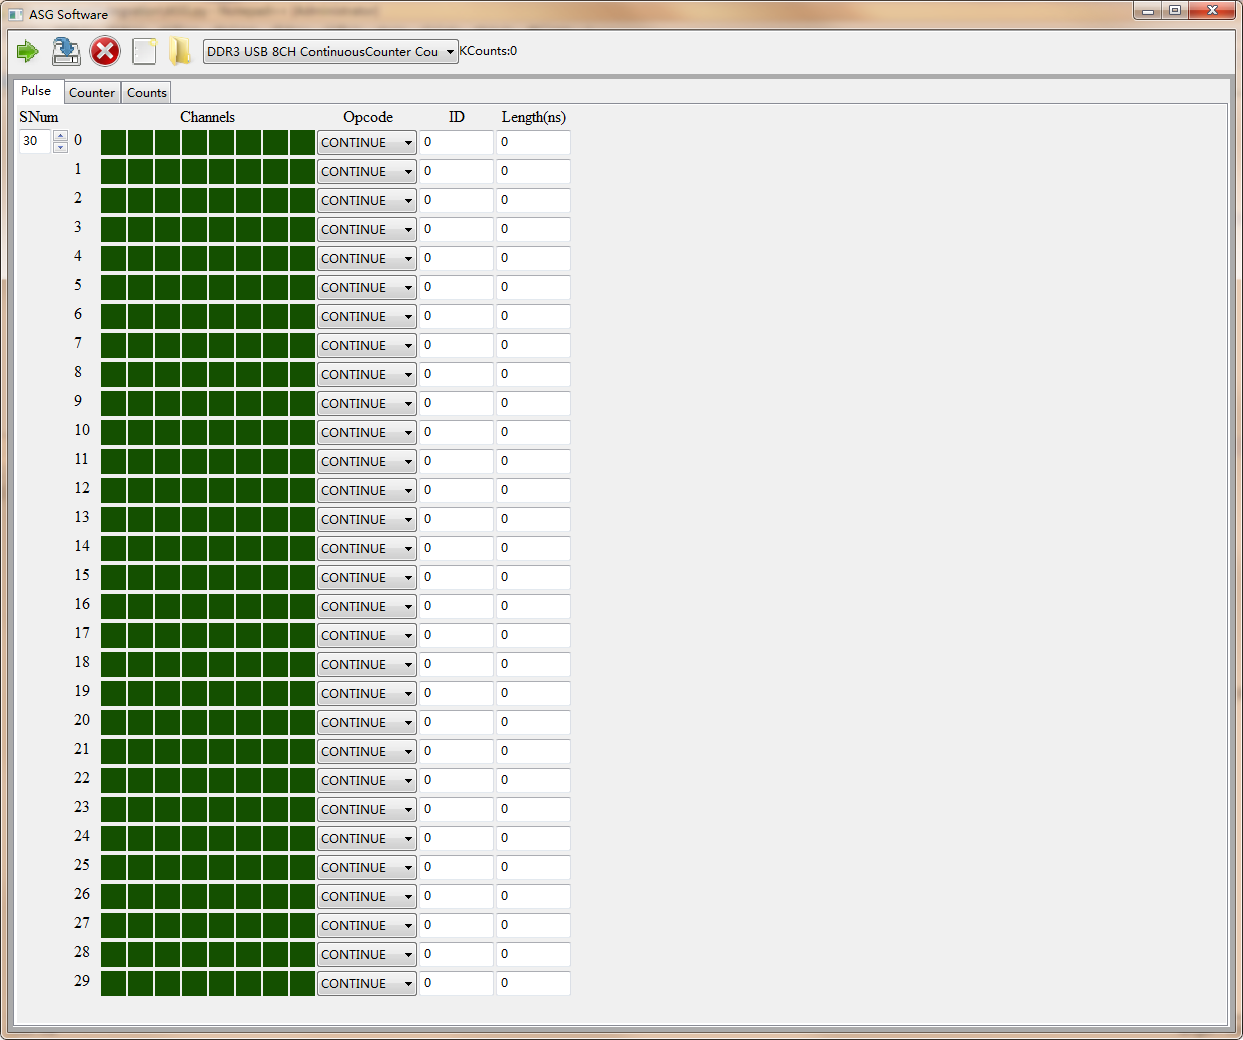
\includegraphics[width=11cm,height=9cm]{fig4_1}
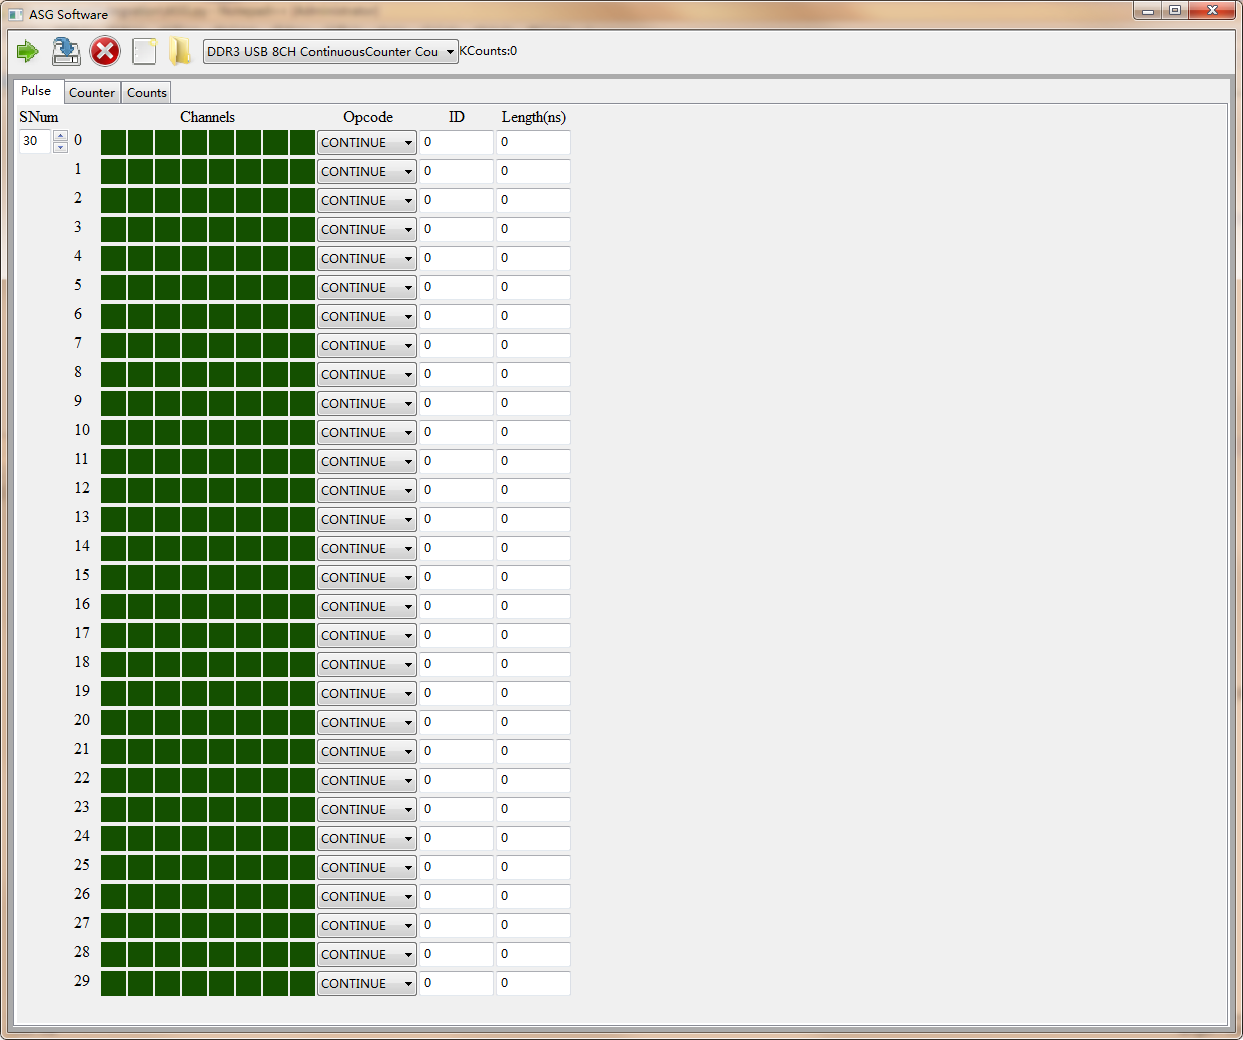
\includegraphics[height=9cm]{fig4_1}
\caption{软件主界面}
\end{figure}

在软件主界面中,每行8个绿色方框,从左往右依次代表OUT 1至OUT 8的8个方波输出通道在一段时间内的输出状态(时间长短由右侧的“Length”文本框内输入的数值决定,单位为纳秒)。当绿色被点亮时,该通道输出高电平;若绿色未被点亮,则该通道输出为低电平。

\section{\heiti 定义任意方波序列}
用户可根据每行绿色方框的不同状态及“Length”的长度来定义任意的方波序列。如用户想要在1、2、3、4通道生成一个高电平宽度为60 ns的方波序列,而5、6、7、8通道在这60 ns内为低电平。则可如图4.2 定义方波序列:
\begin{figure}[ht]
\centering
%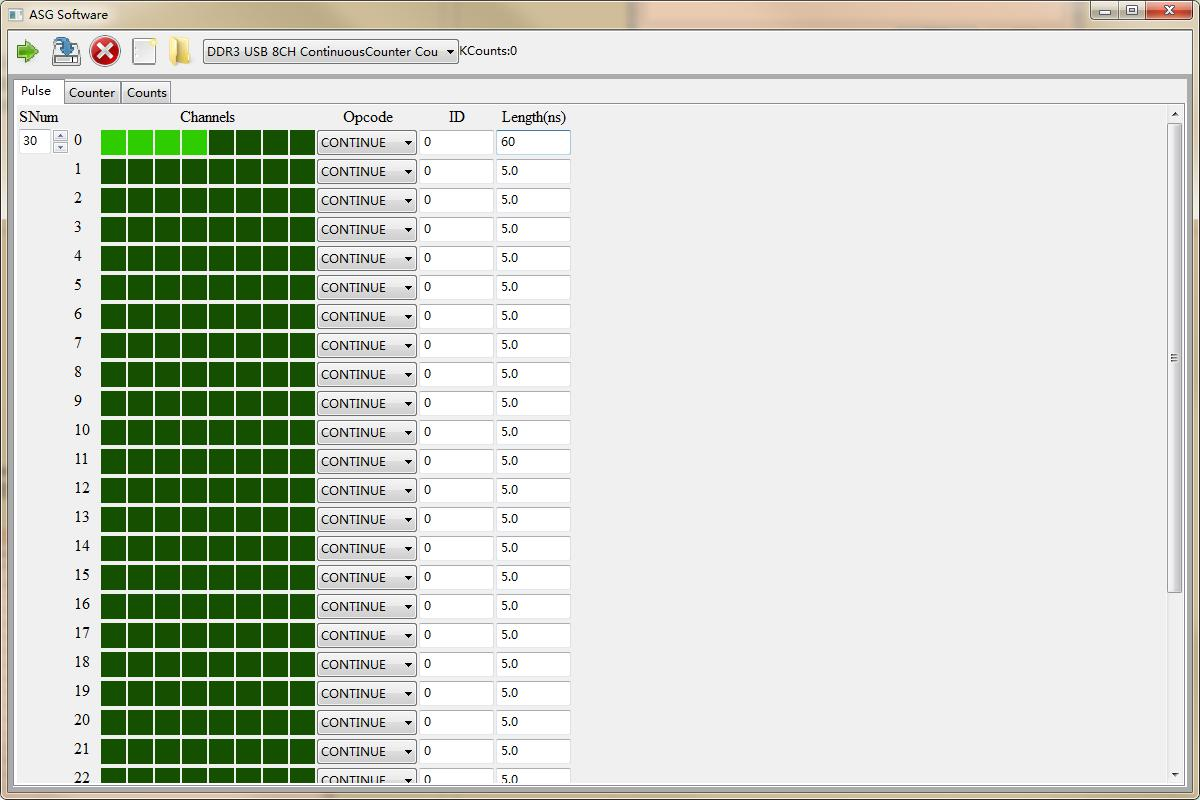
\includegraphics[width=11cm,height=9cm]{fig4_2}
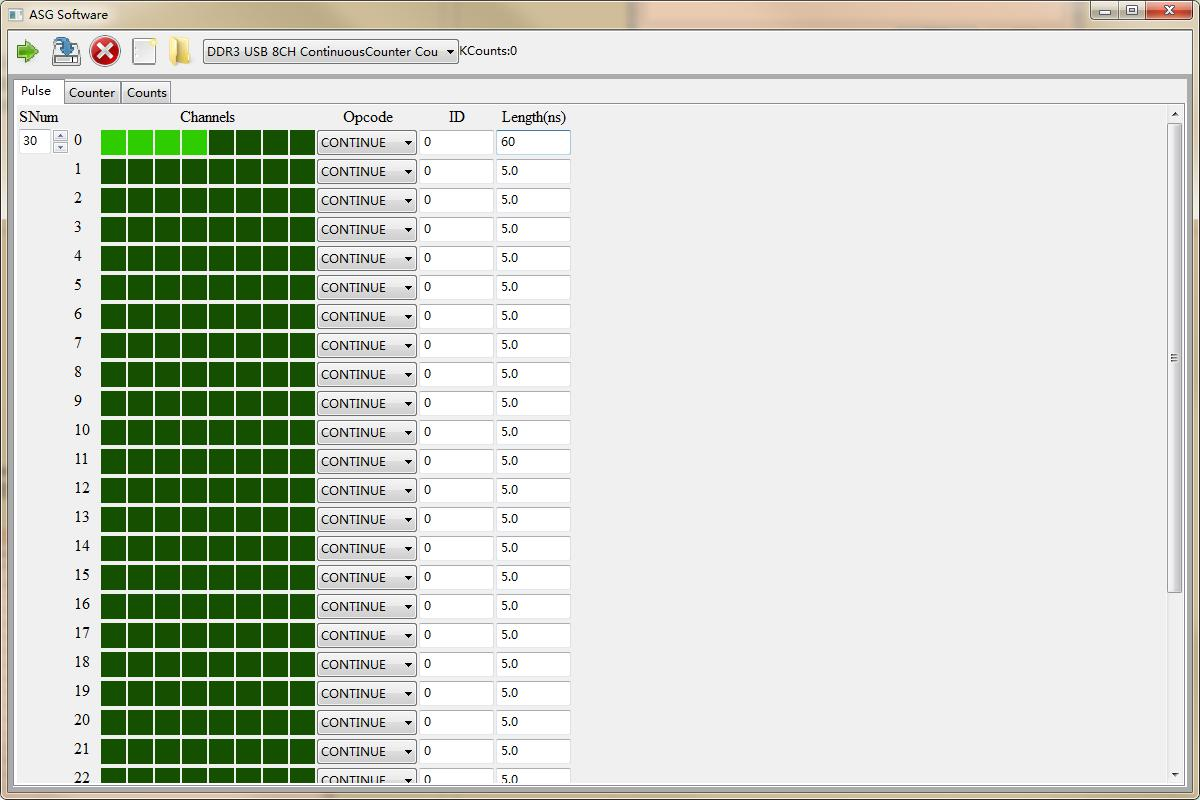
\includegraphics[height=9cm]{fig4_2}
\caption{自定义方波序列}
\end{figure}

\section{\heiti 定义方波序列注意事项}
\noindent \textbf{(1)}. 每个通道的方波序列中单个方波脉冲高低电平时间必须在7.5 ns至2.6 s以内。如用户定义的方波序列中存在单个脉冲宽度小于7.5 ns 的情况,则为非法输入,如图4.3。
\begin{figure}[H]
\centering
%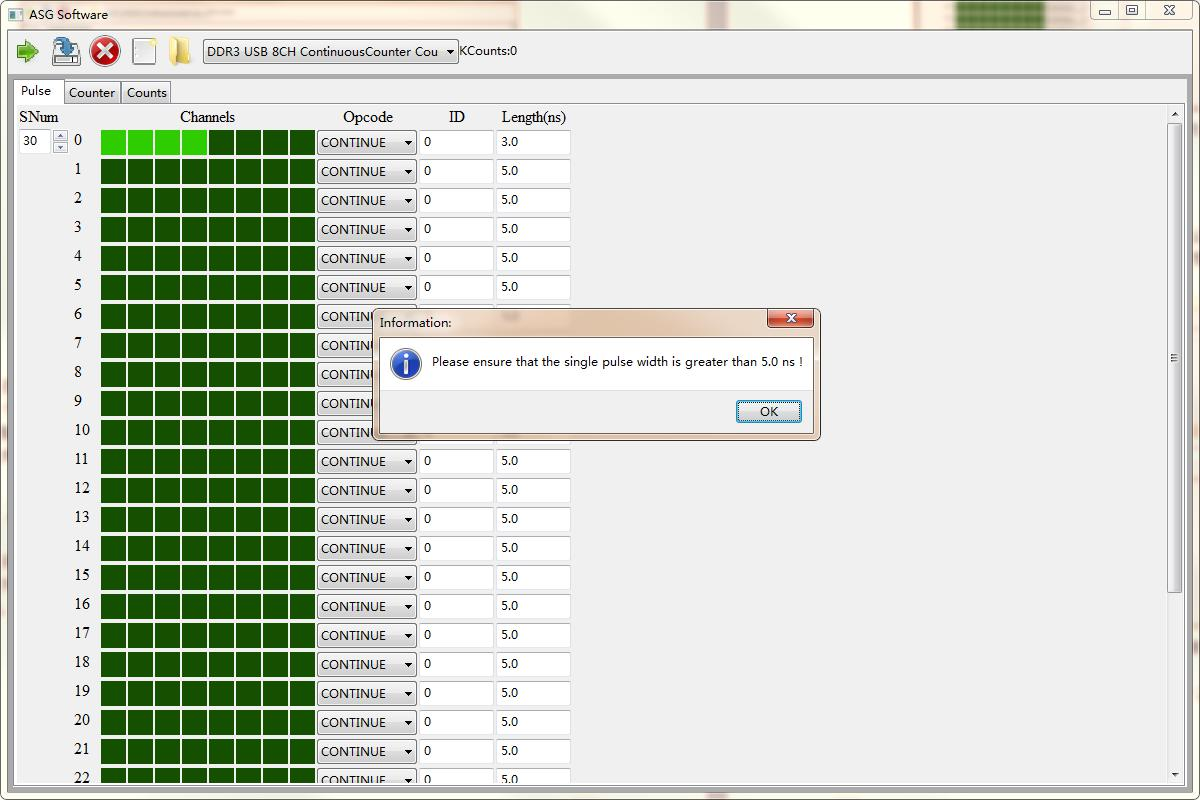
\includegraphics[width=11cm,height=9cm]{fig4_3}
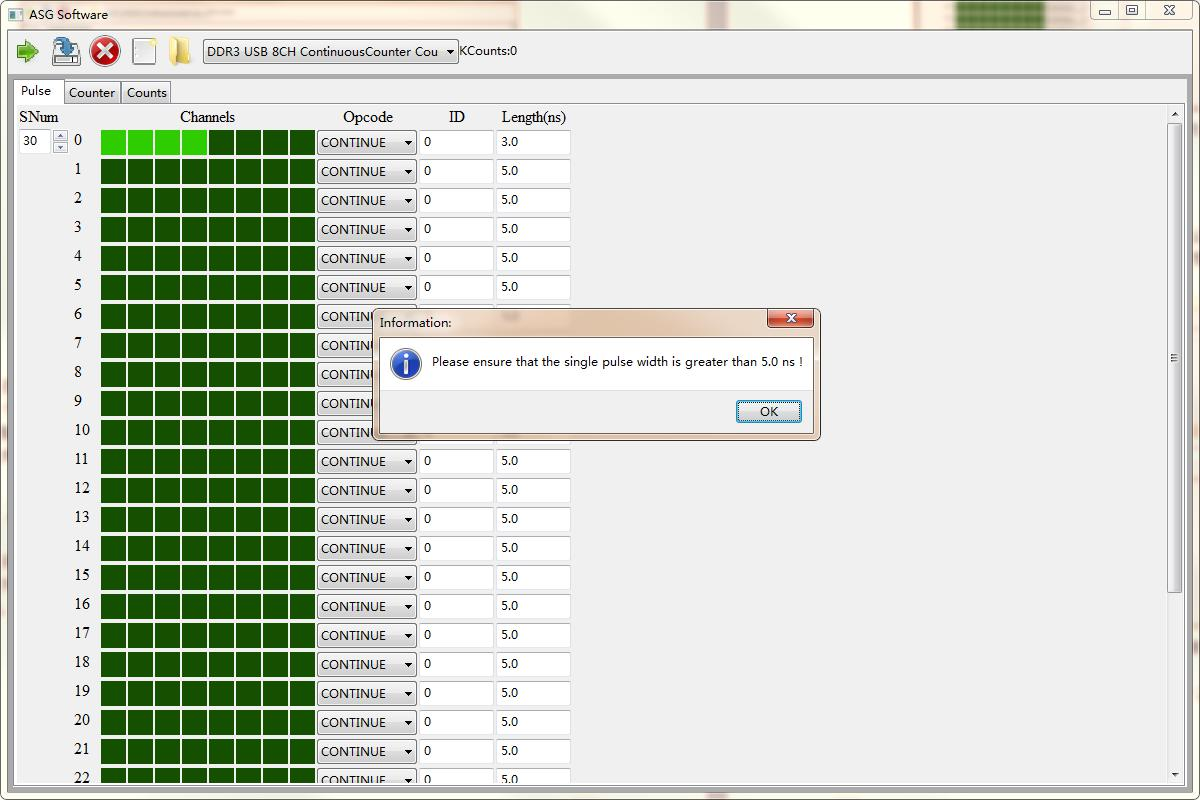
\includegraphics[height=9cm]{fig4_3}
\caption{宽度小于7.5 ns的非法方波序列输入}
\end{figure}

\newpage
\noindent \textbf{(2)}.  若用户定义的方波序列中存在单个脉冲宽度大于2.6 s的情况,亦为非法输入,如图4.4。
\begin{figure}[ht]
\centering
%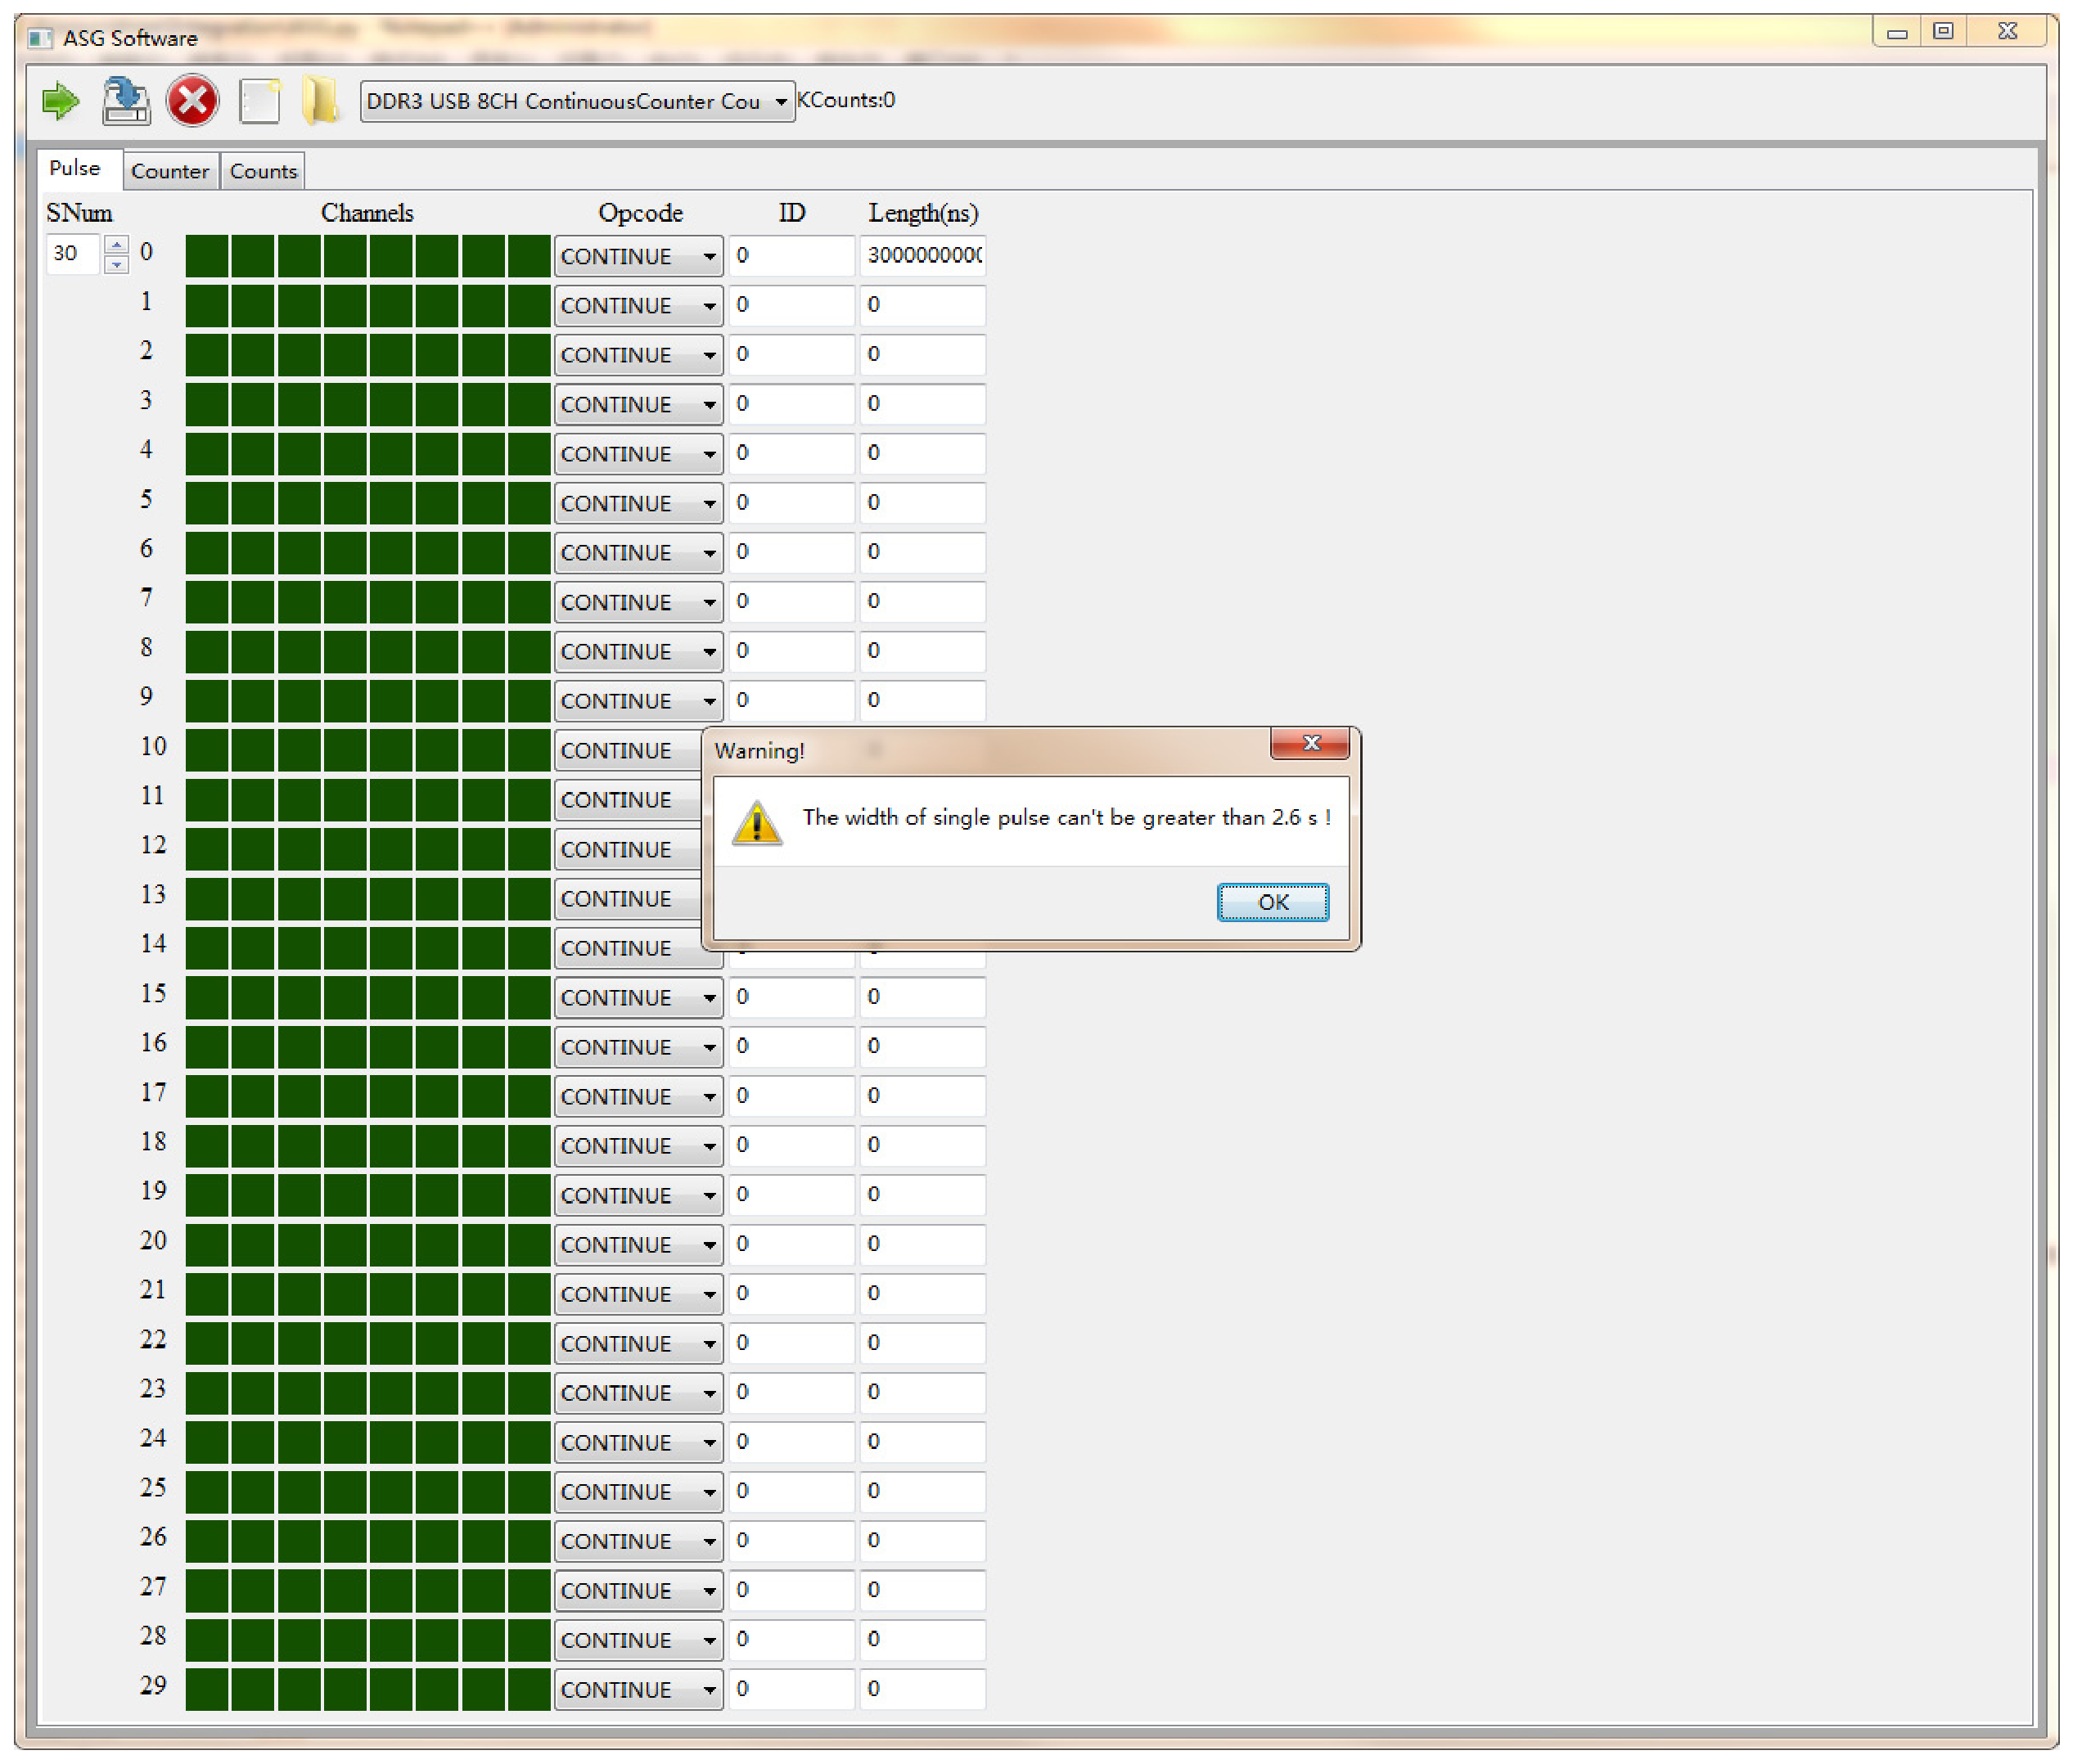
\includegraphics[width=11cm,height=9cm]{fig4_4}
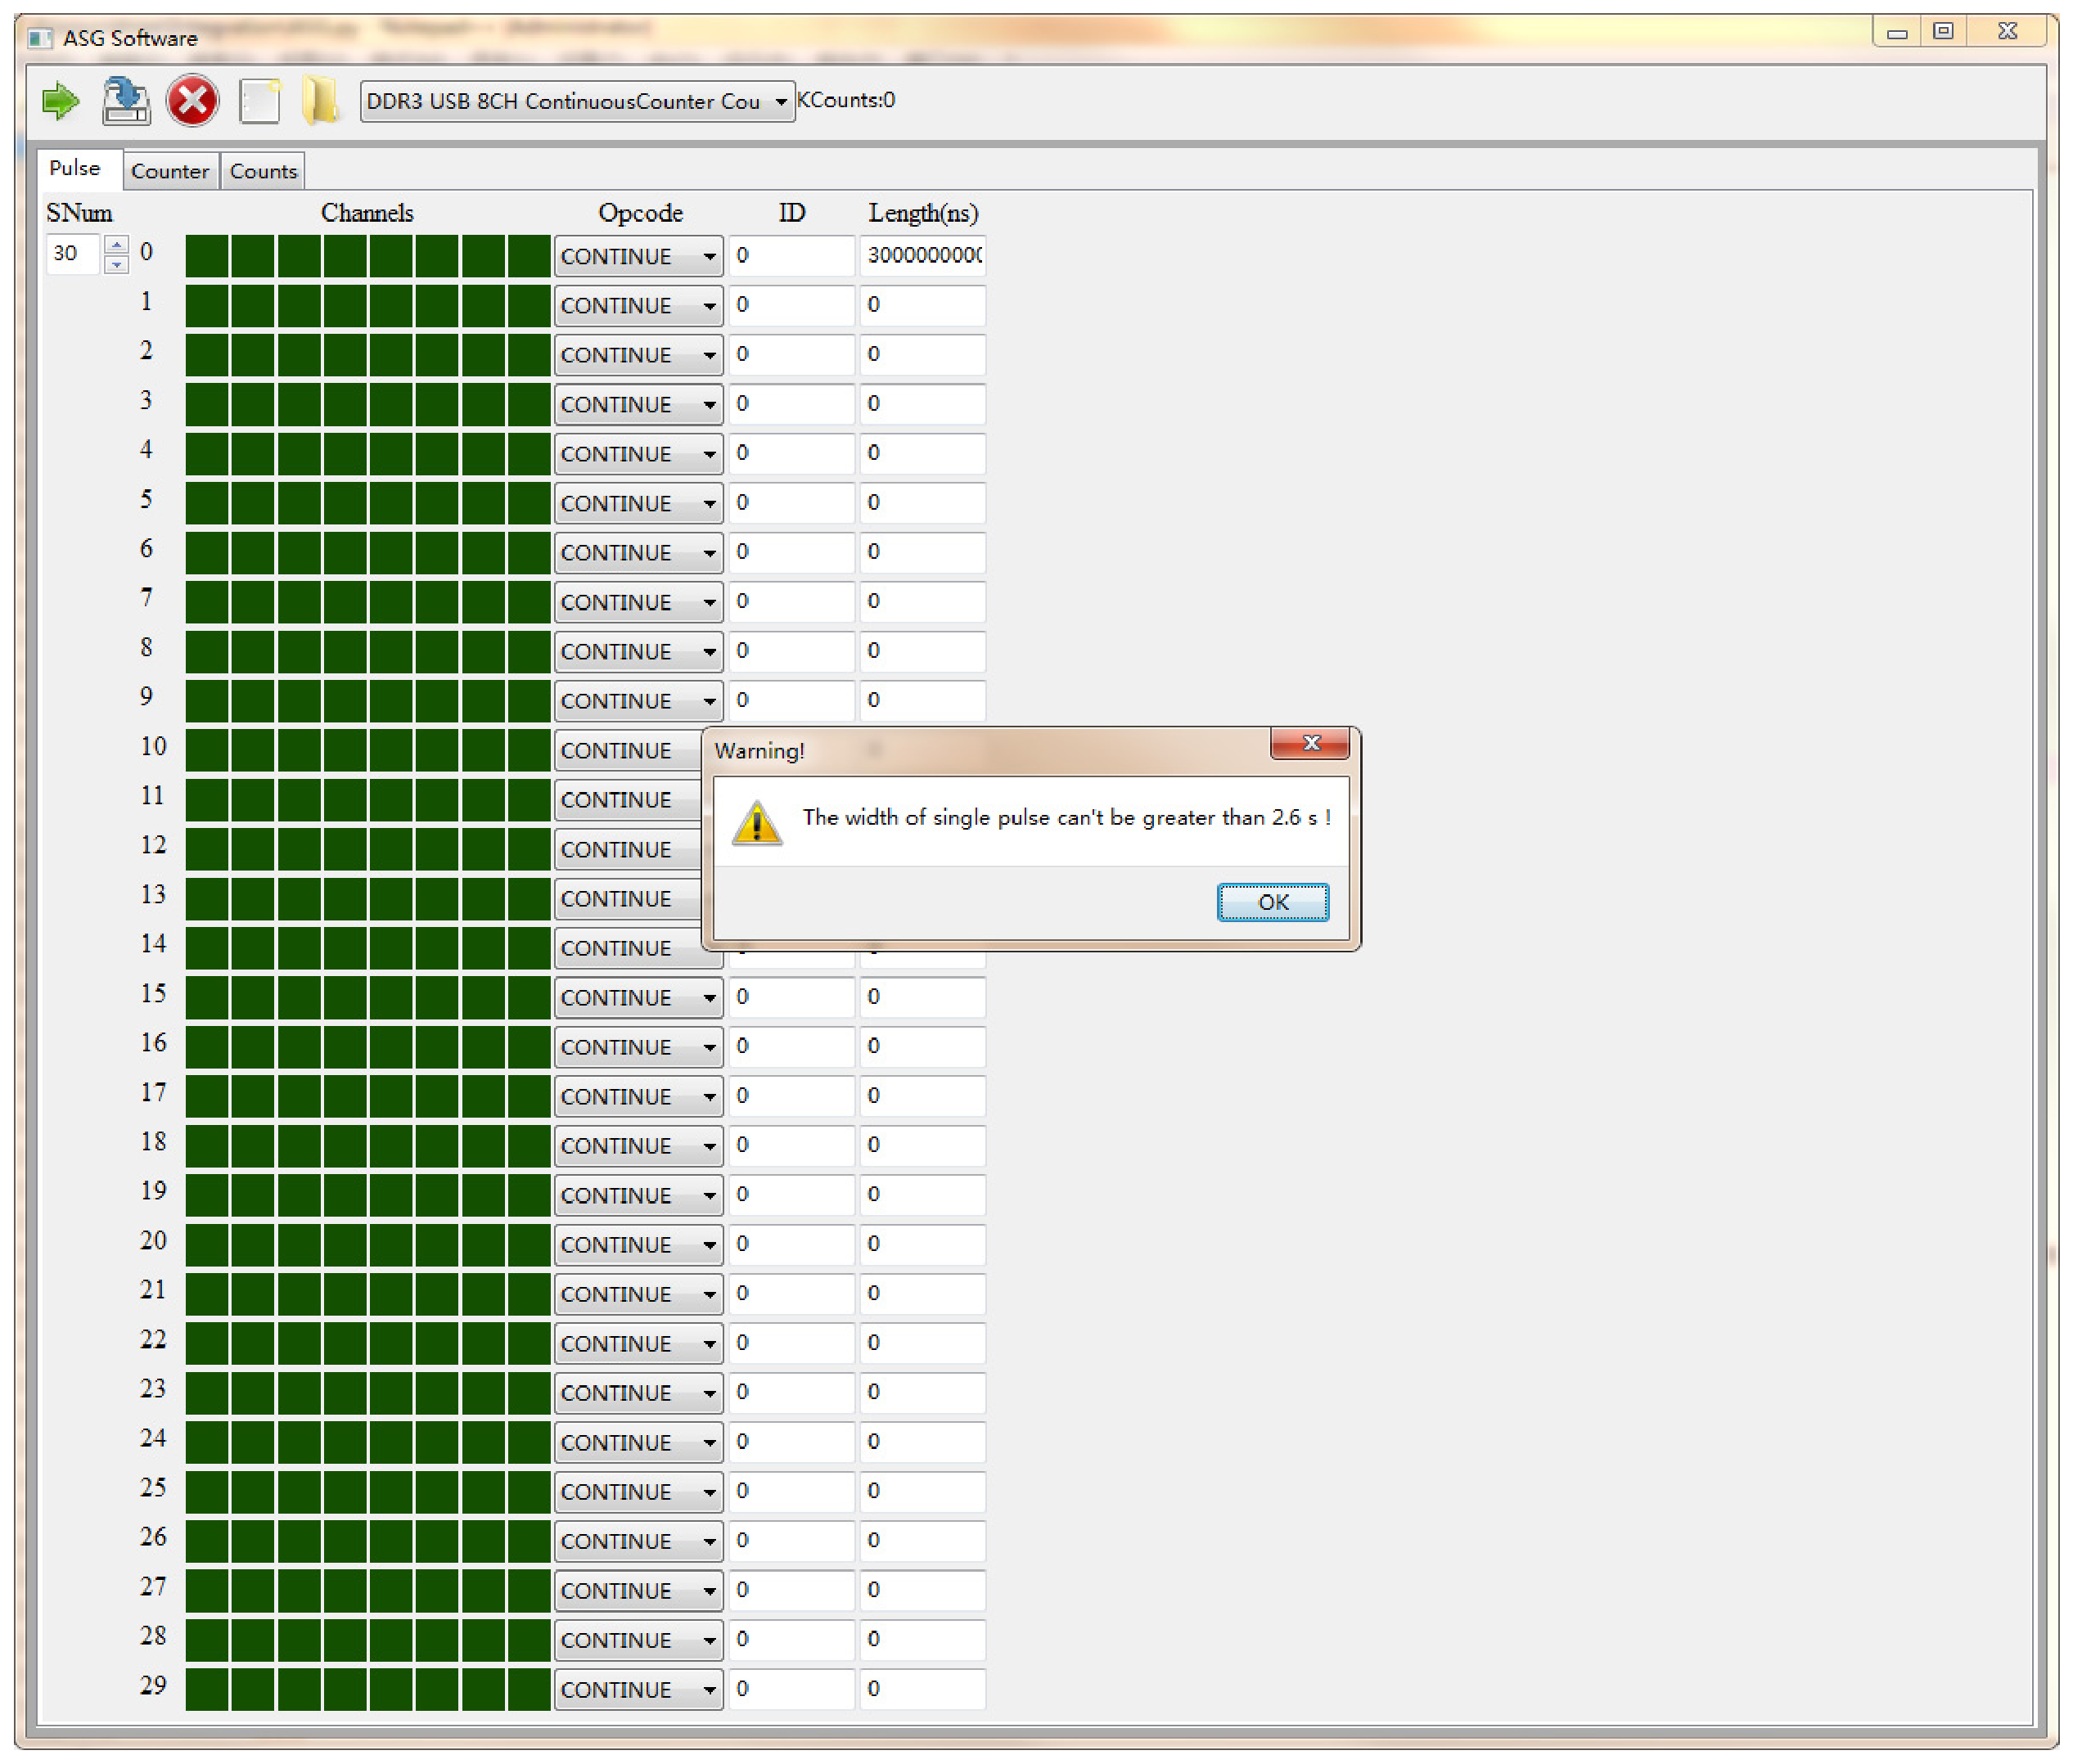
\includegraphics[height=9cm]{fig4_4}
\caption{宽度大于2.6 s的非法方波序列输入}
\end{figure}

\noindent \textbf{(3)}. 用户定义的每个方波脉冲宽度必须是0.05 ns的整数倍,若存在非0.05 ns整数倍的情况,亦为非法输入,如图4.5。
\begin{figure}[H]
\centering
%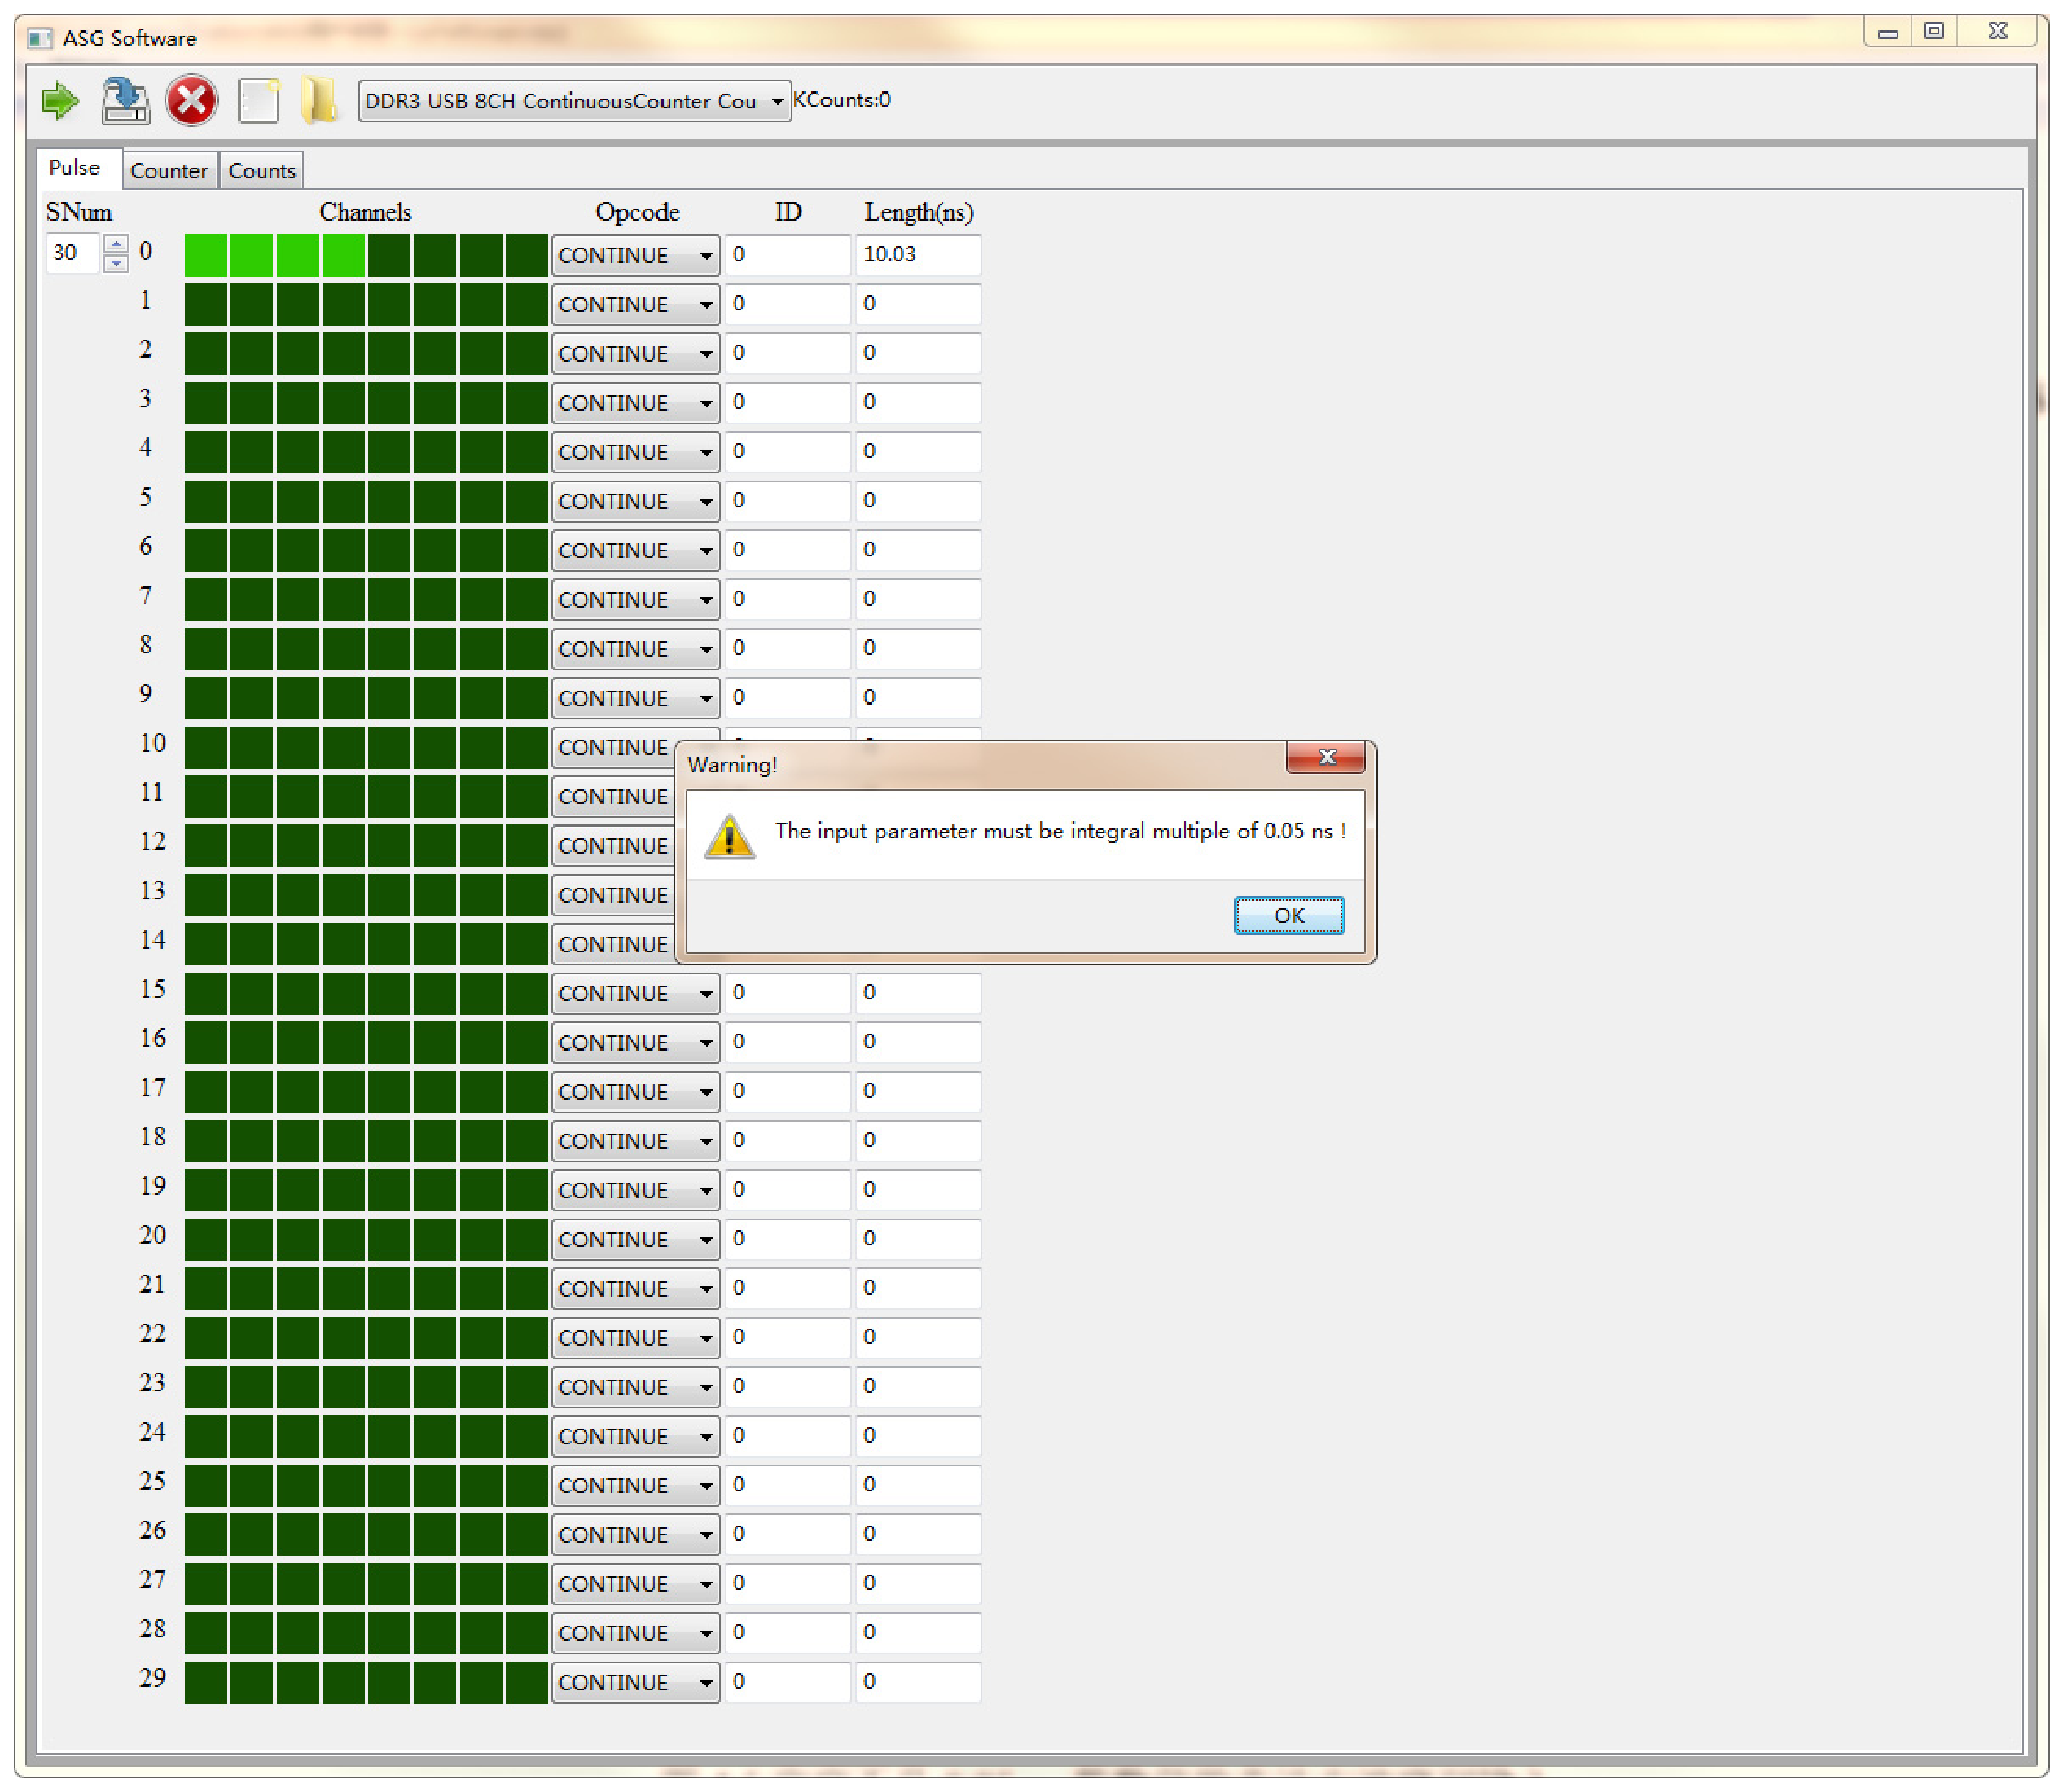
\includegraphics[width=11cm,height=9cm]{fig4_5}
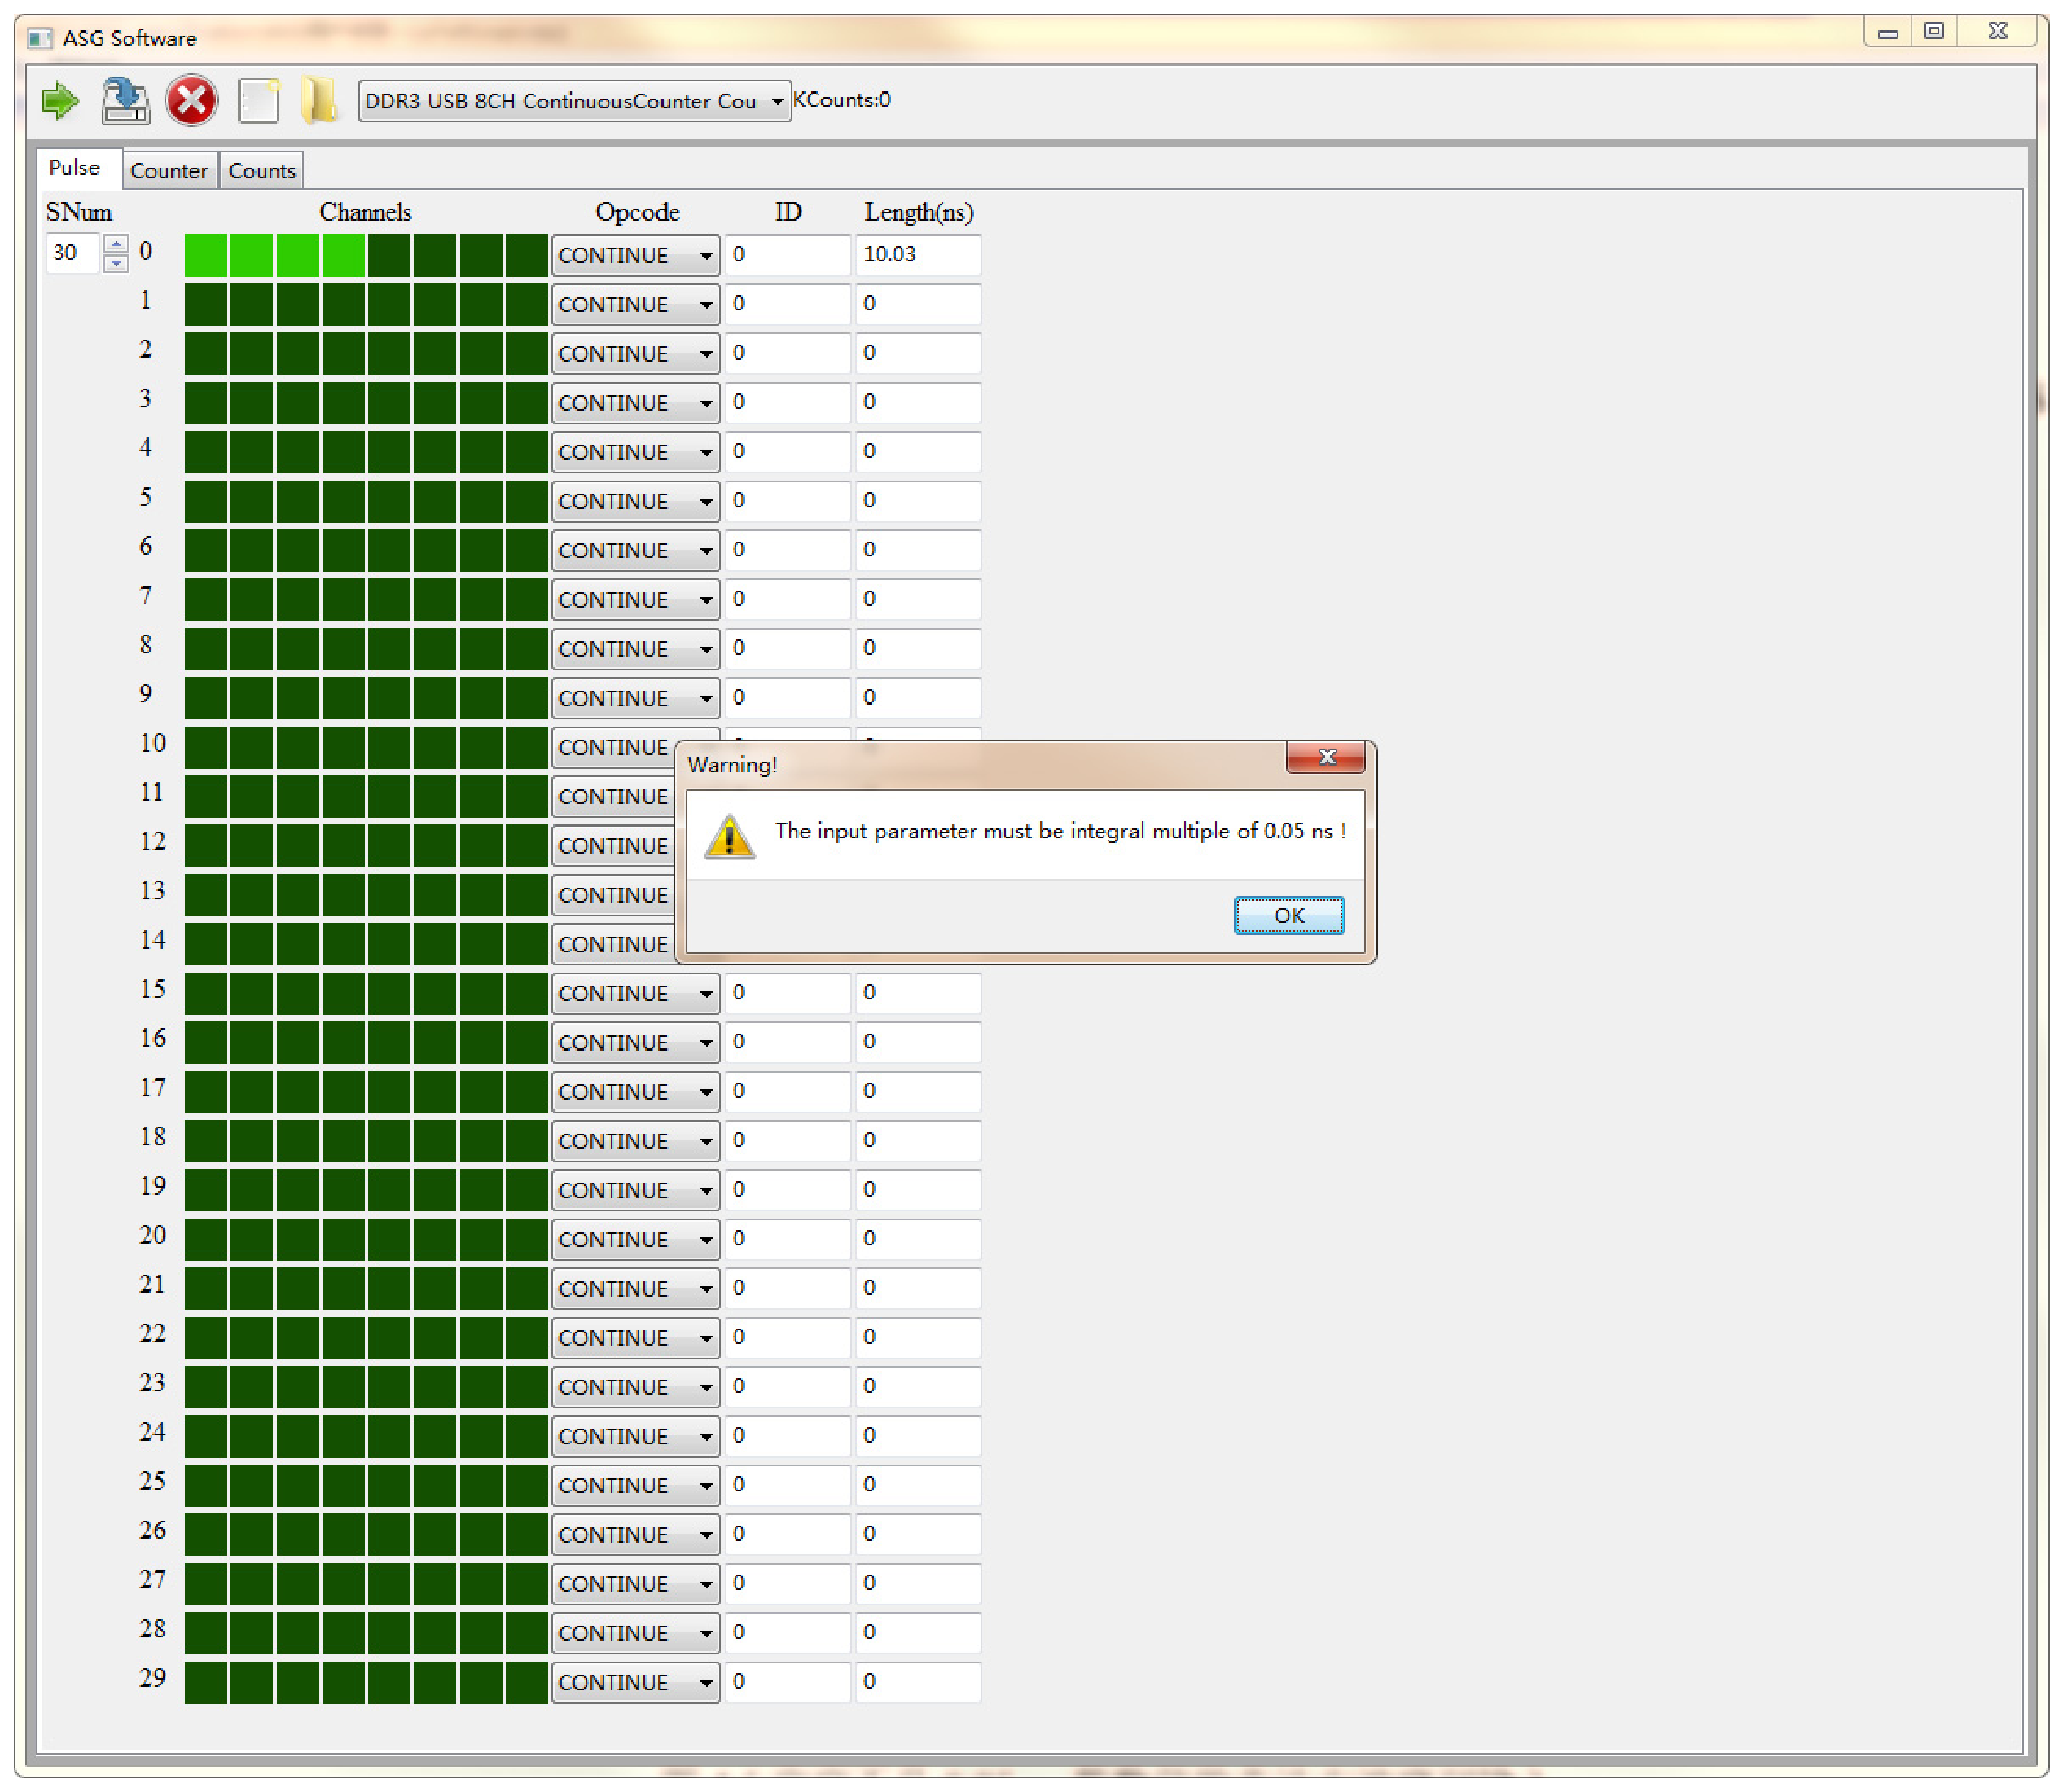
\includegraphics[height=9cm]{fig4_5}
\caption{宽度不是0.05 ns整数倍的非法方波序列输入}
\end{figure}

\section{\heiti{定义}计数通道使能\heiti{序列}}
用户选择“Counter”选项卡进入定义计数通道使能序列界面,如图4.6。左侧为显示计数结果的坐标图。用户可根据中间绿色方框的状态以及“Length”的长度来定义任意的计数通道使能序列。同方波序列输入,绿色方框被点亮代表高电平,未点亮代表低电平。
\begin{figure}[ht]
\centering
%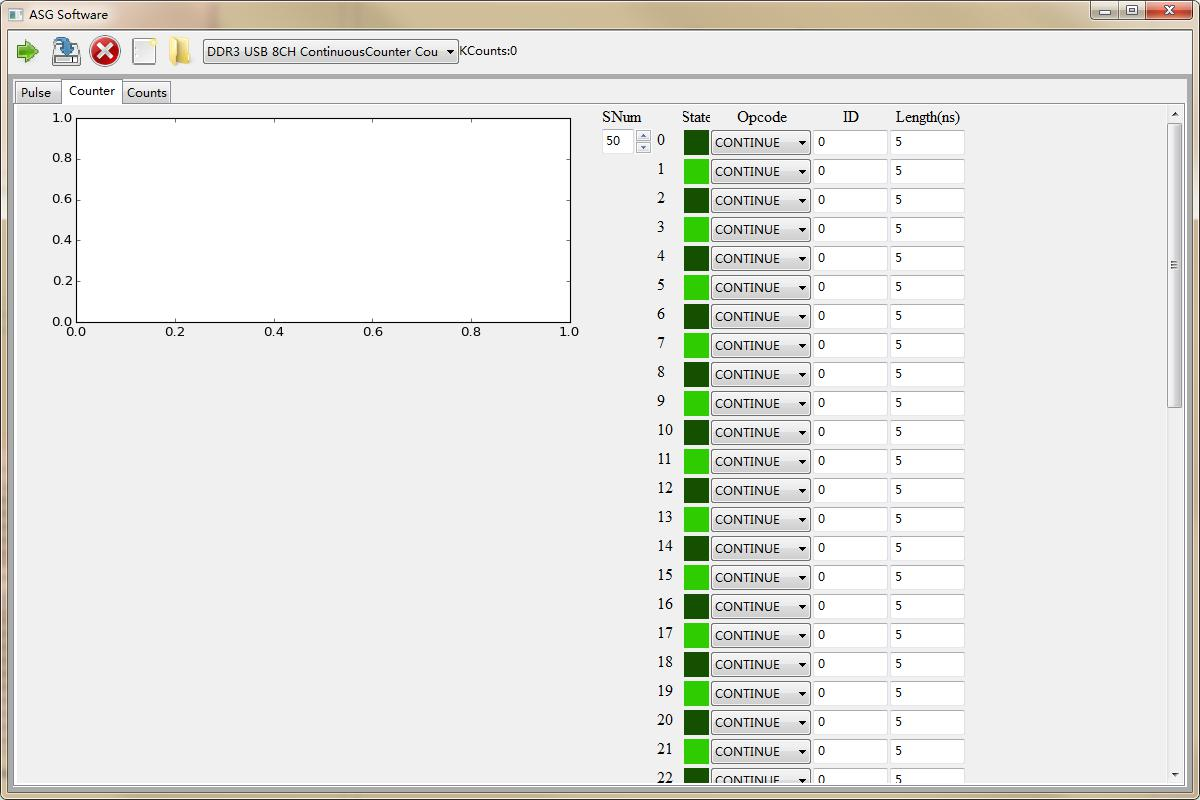
\includegraphics[width=10cm,height=8cm]{fig4_6}
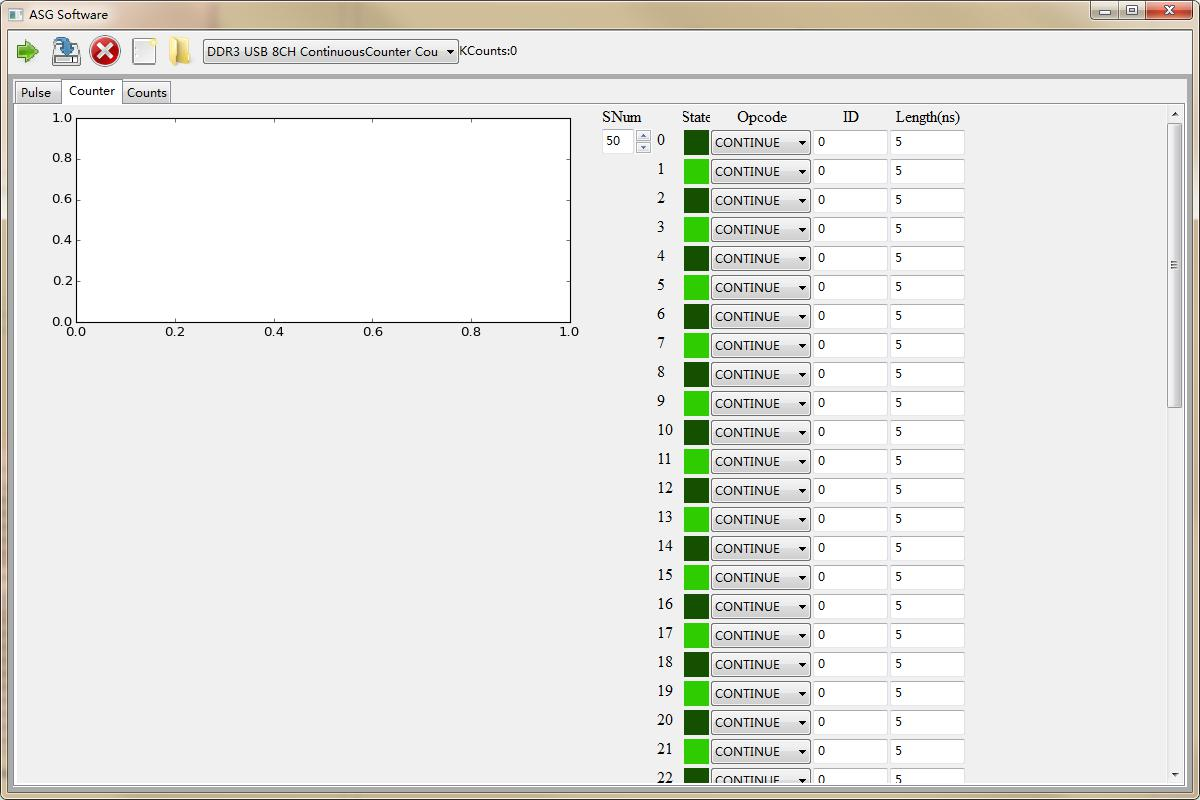
\includegraphics[height=9cm]{fig4_6}
\caption{Counter 界面}
\end{figure}

\section{\heiti{定义}计数通道使能\heiti{序列注意事项}}
\noindent \textbf{(1)}.  单个计数通道使能序列的高低电平时间必须在5 ns至5000 s以内。如用户定义的计数通道使能序列中存在宽度小于5 ns的情况,则为非法输入,如图4.7。
\begin{figure}[ht]
\centering
%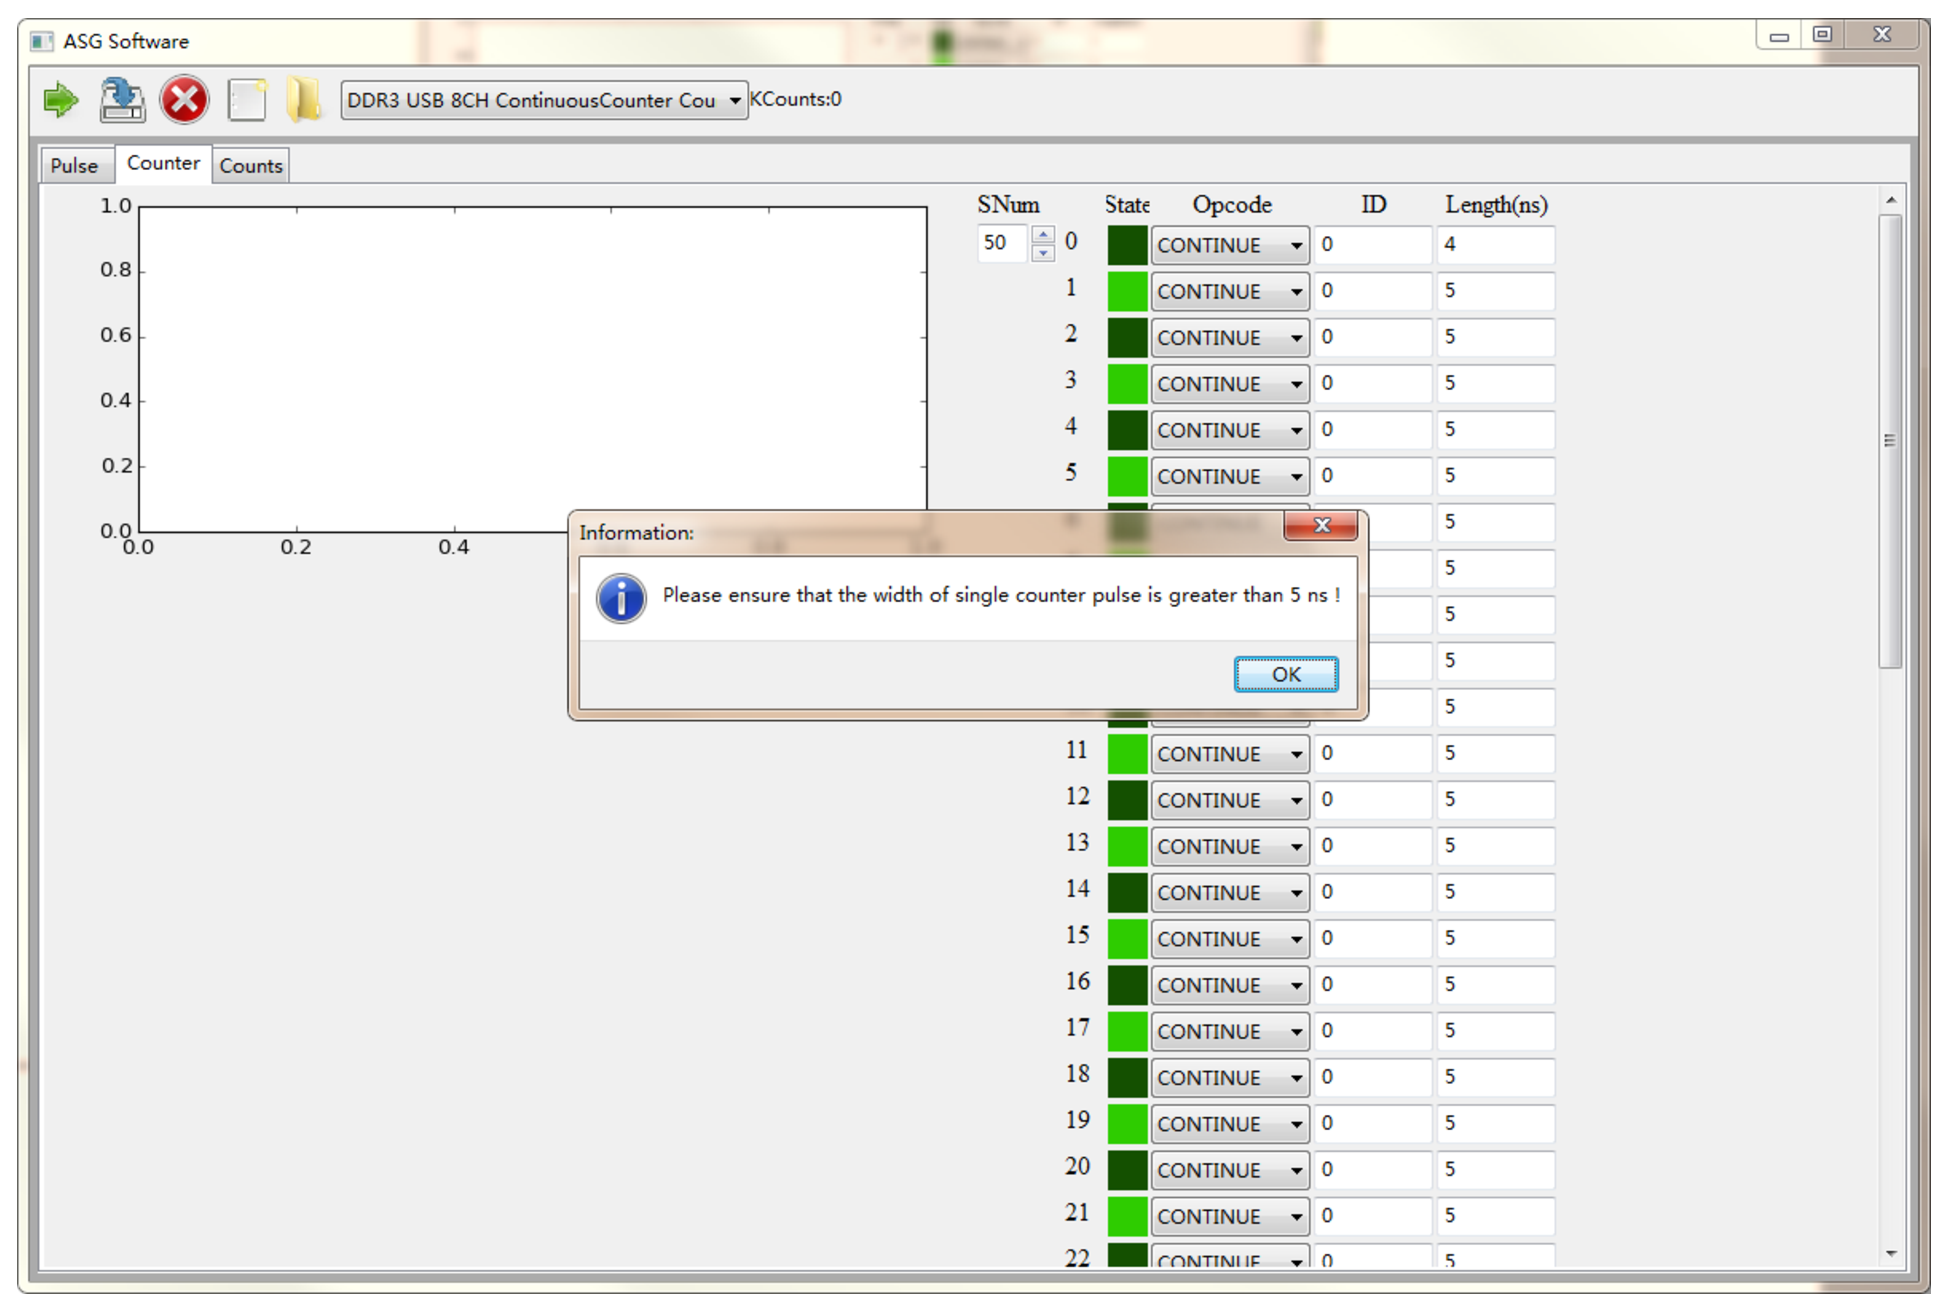
\includegraphics[width=10cm,height=8cm]{fig4_7}
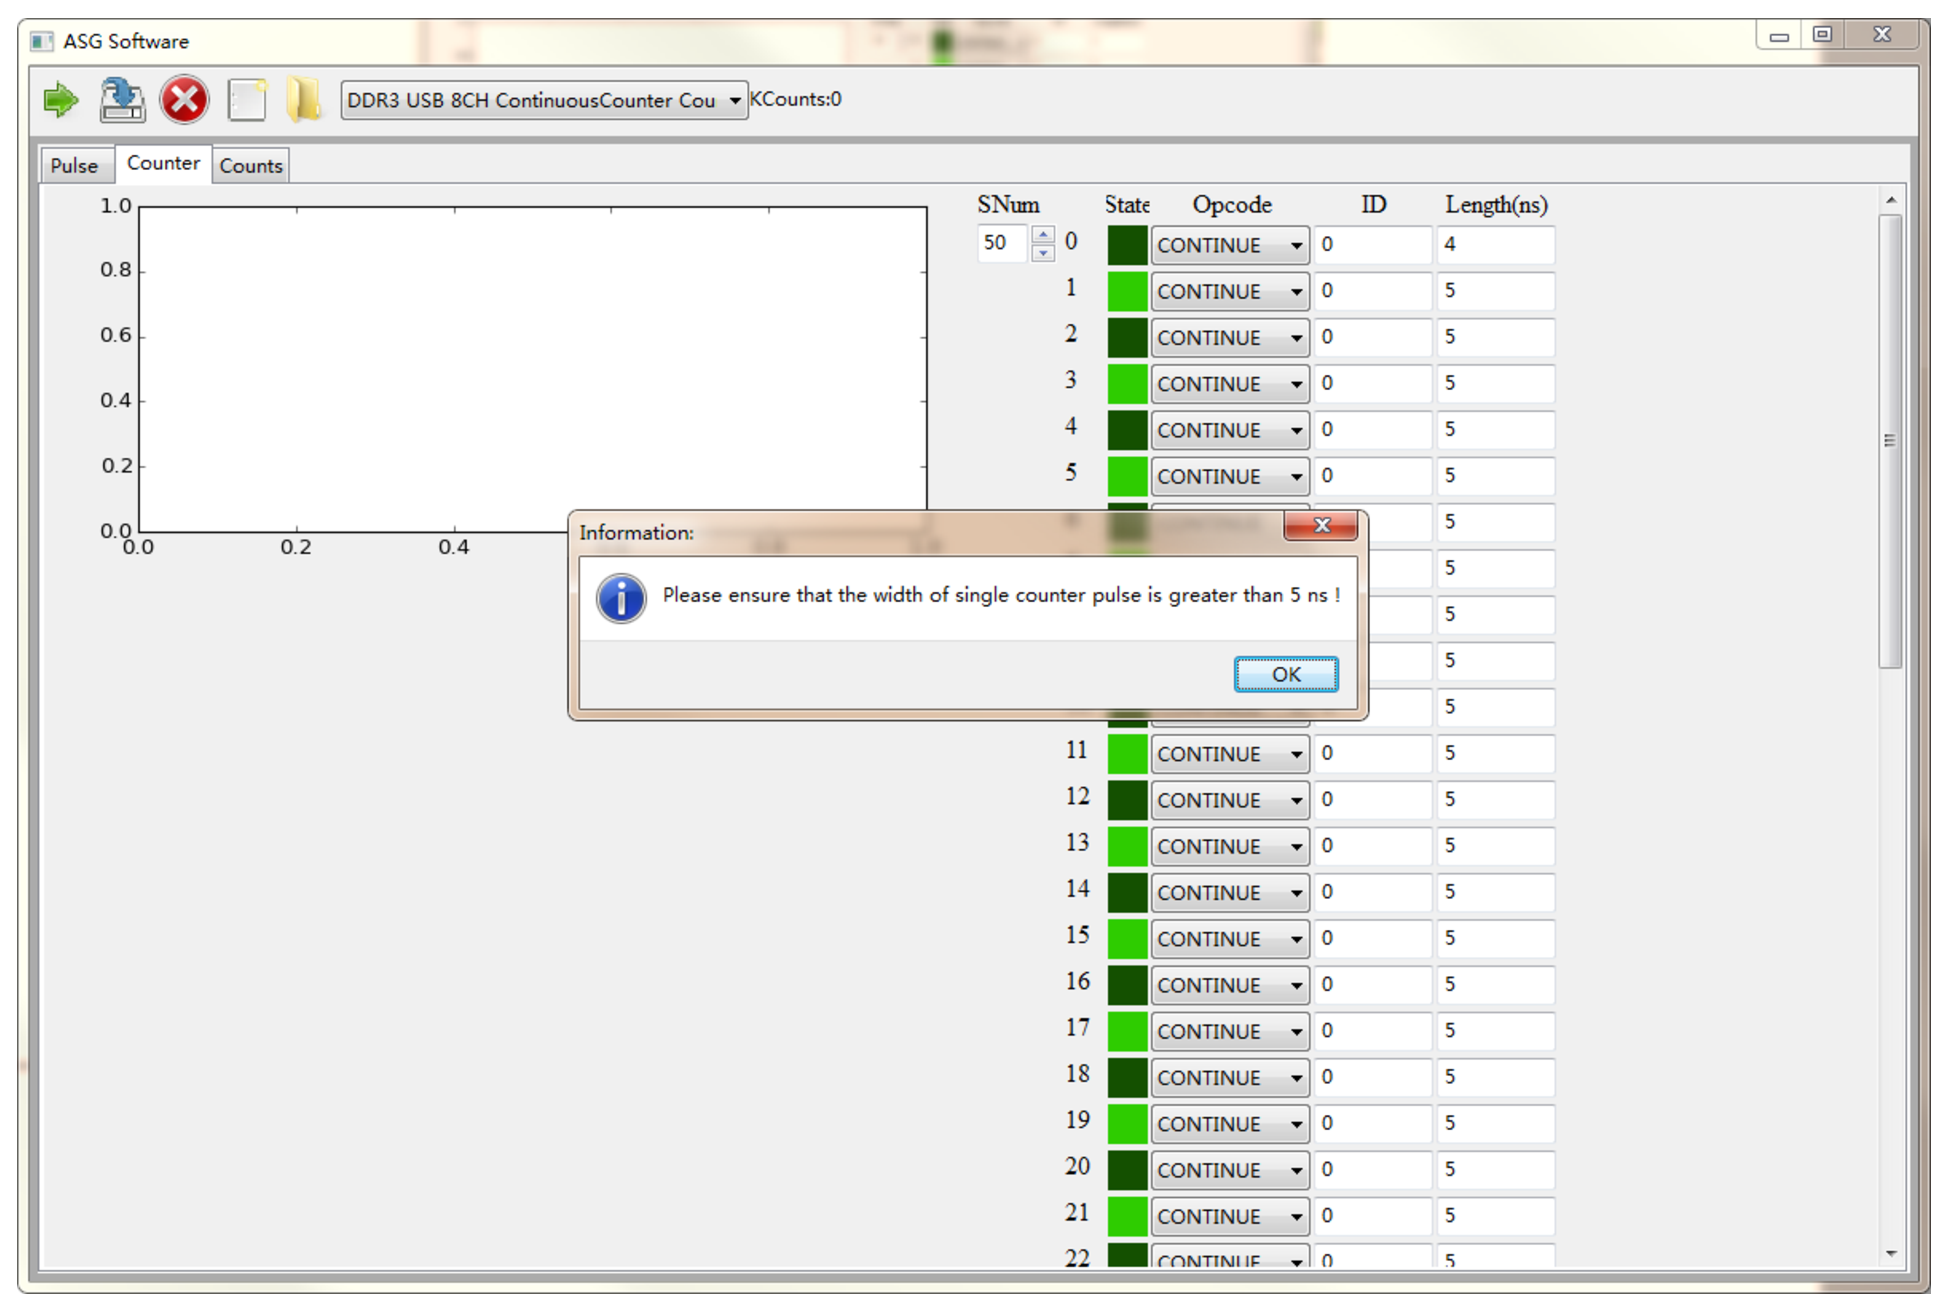
\includegraphics[height=8cm]{fig4_7}
\caption{宽度小于5 ns的非法计数通道使能序列输入}
\end{figure}

\newpage
\noindent \textbf{(2)}.  若用户定义的计数通道使能序列中存在宽度大于5000 s的情况,亦为非法输入,如图4.8。
\begin{figure}[ht]
\centering
%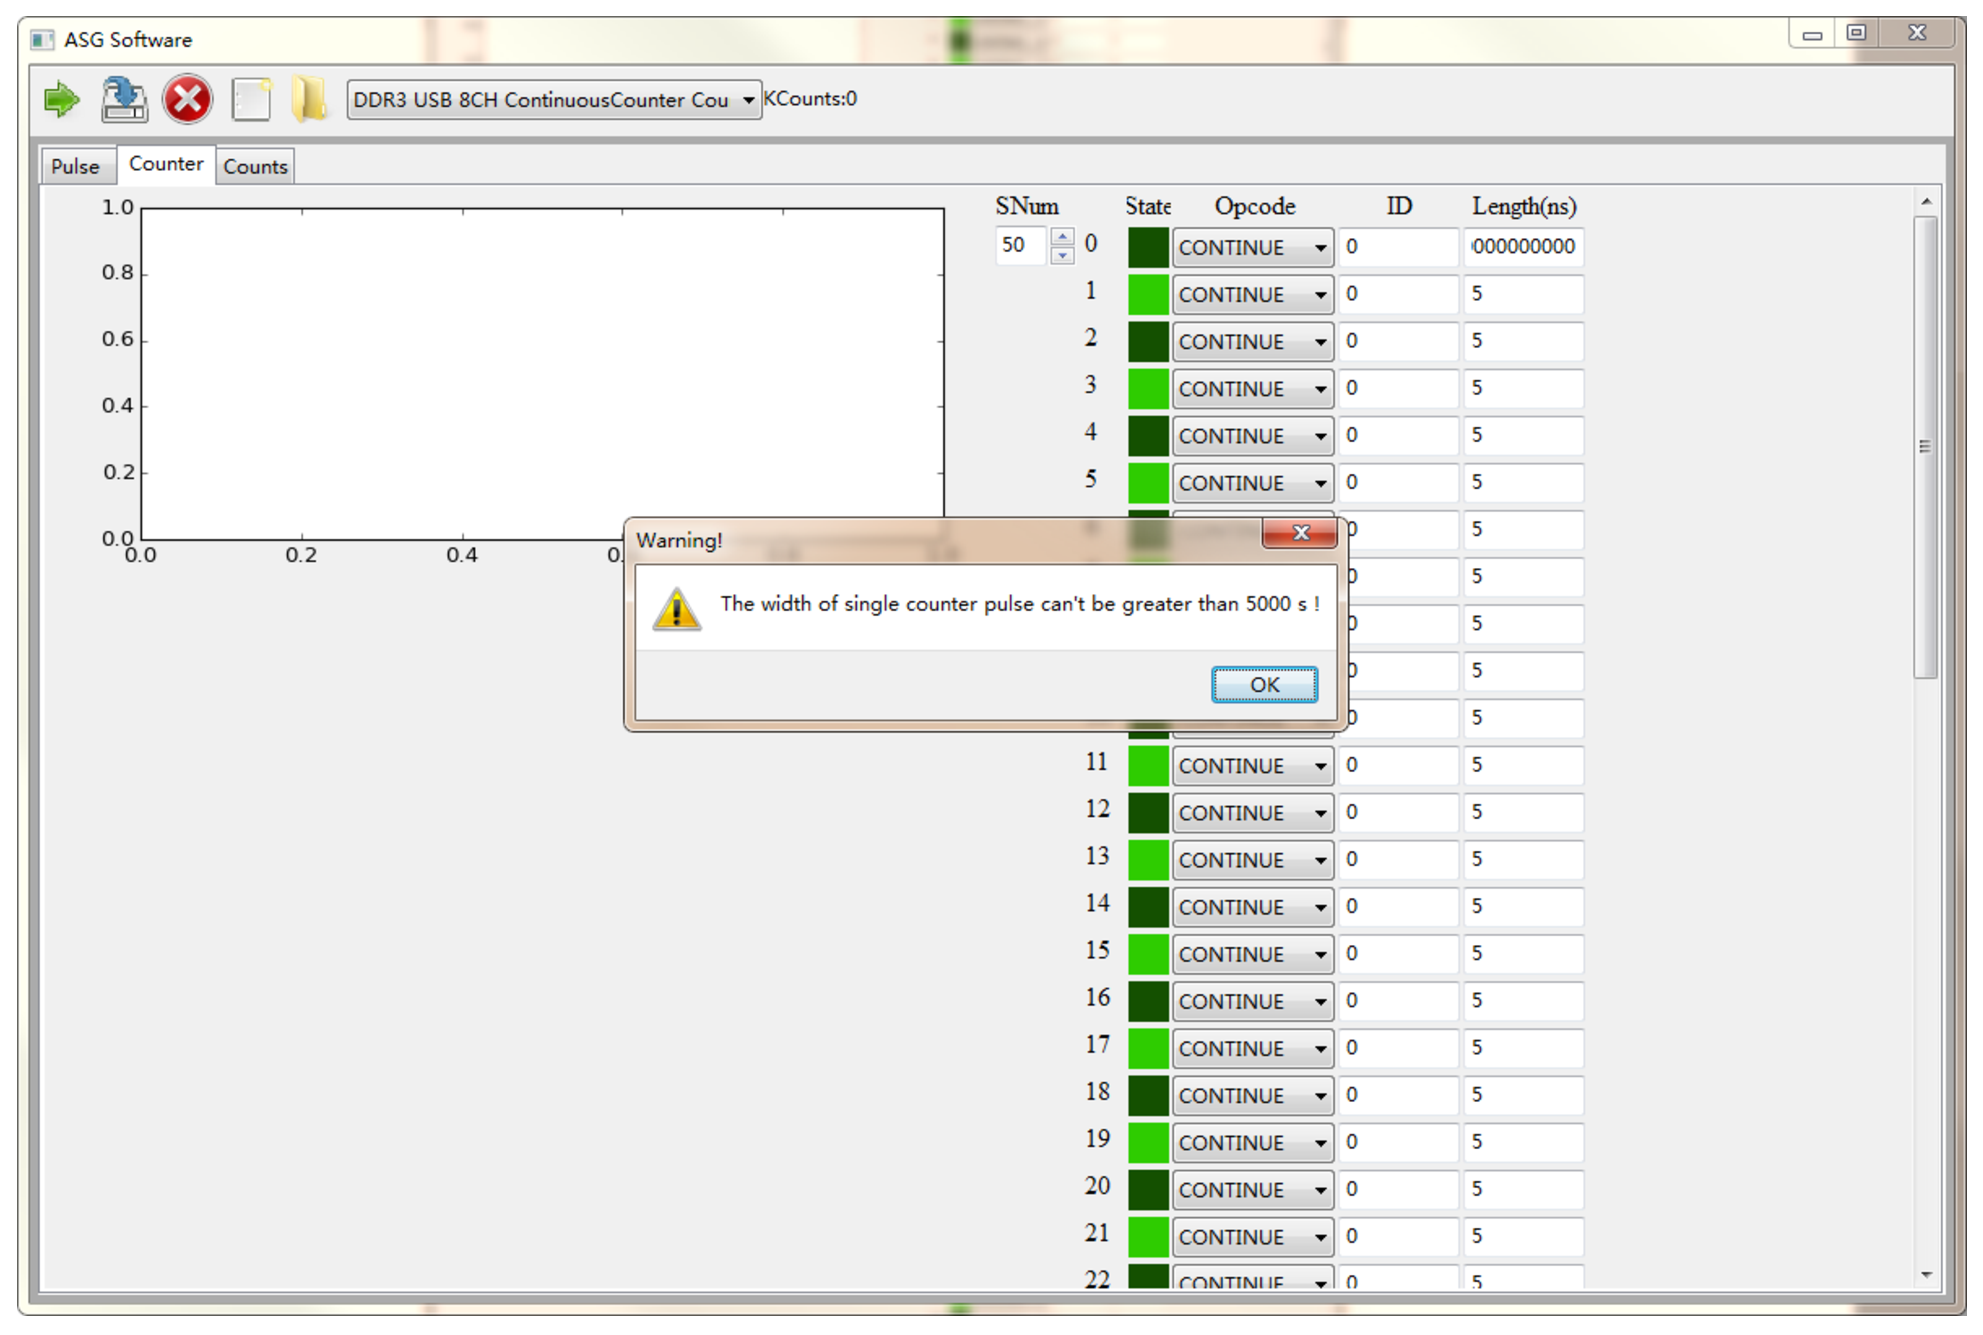
\includegraphics[width=10cm,height=7.5cm]{fig4_8}
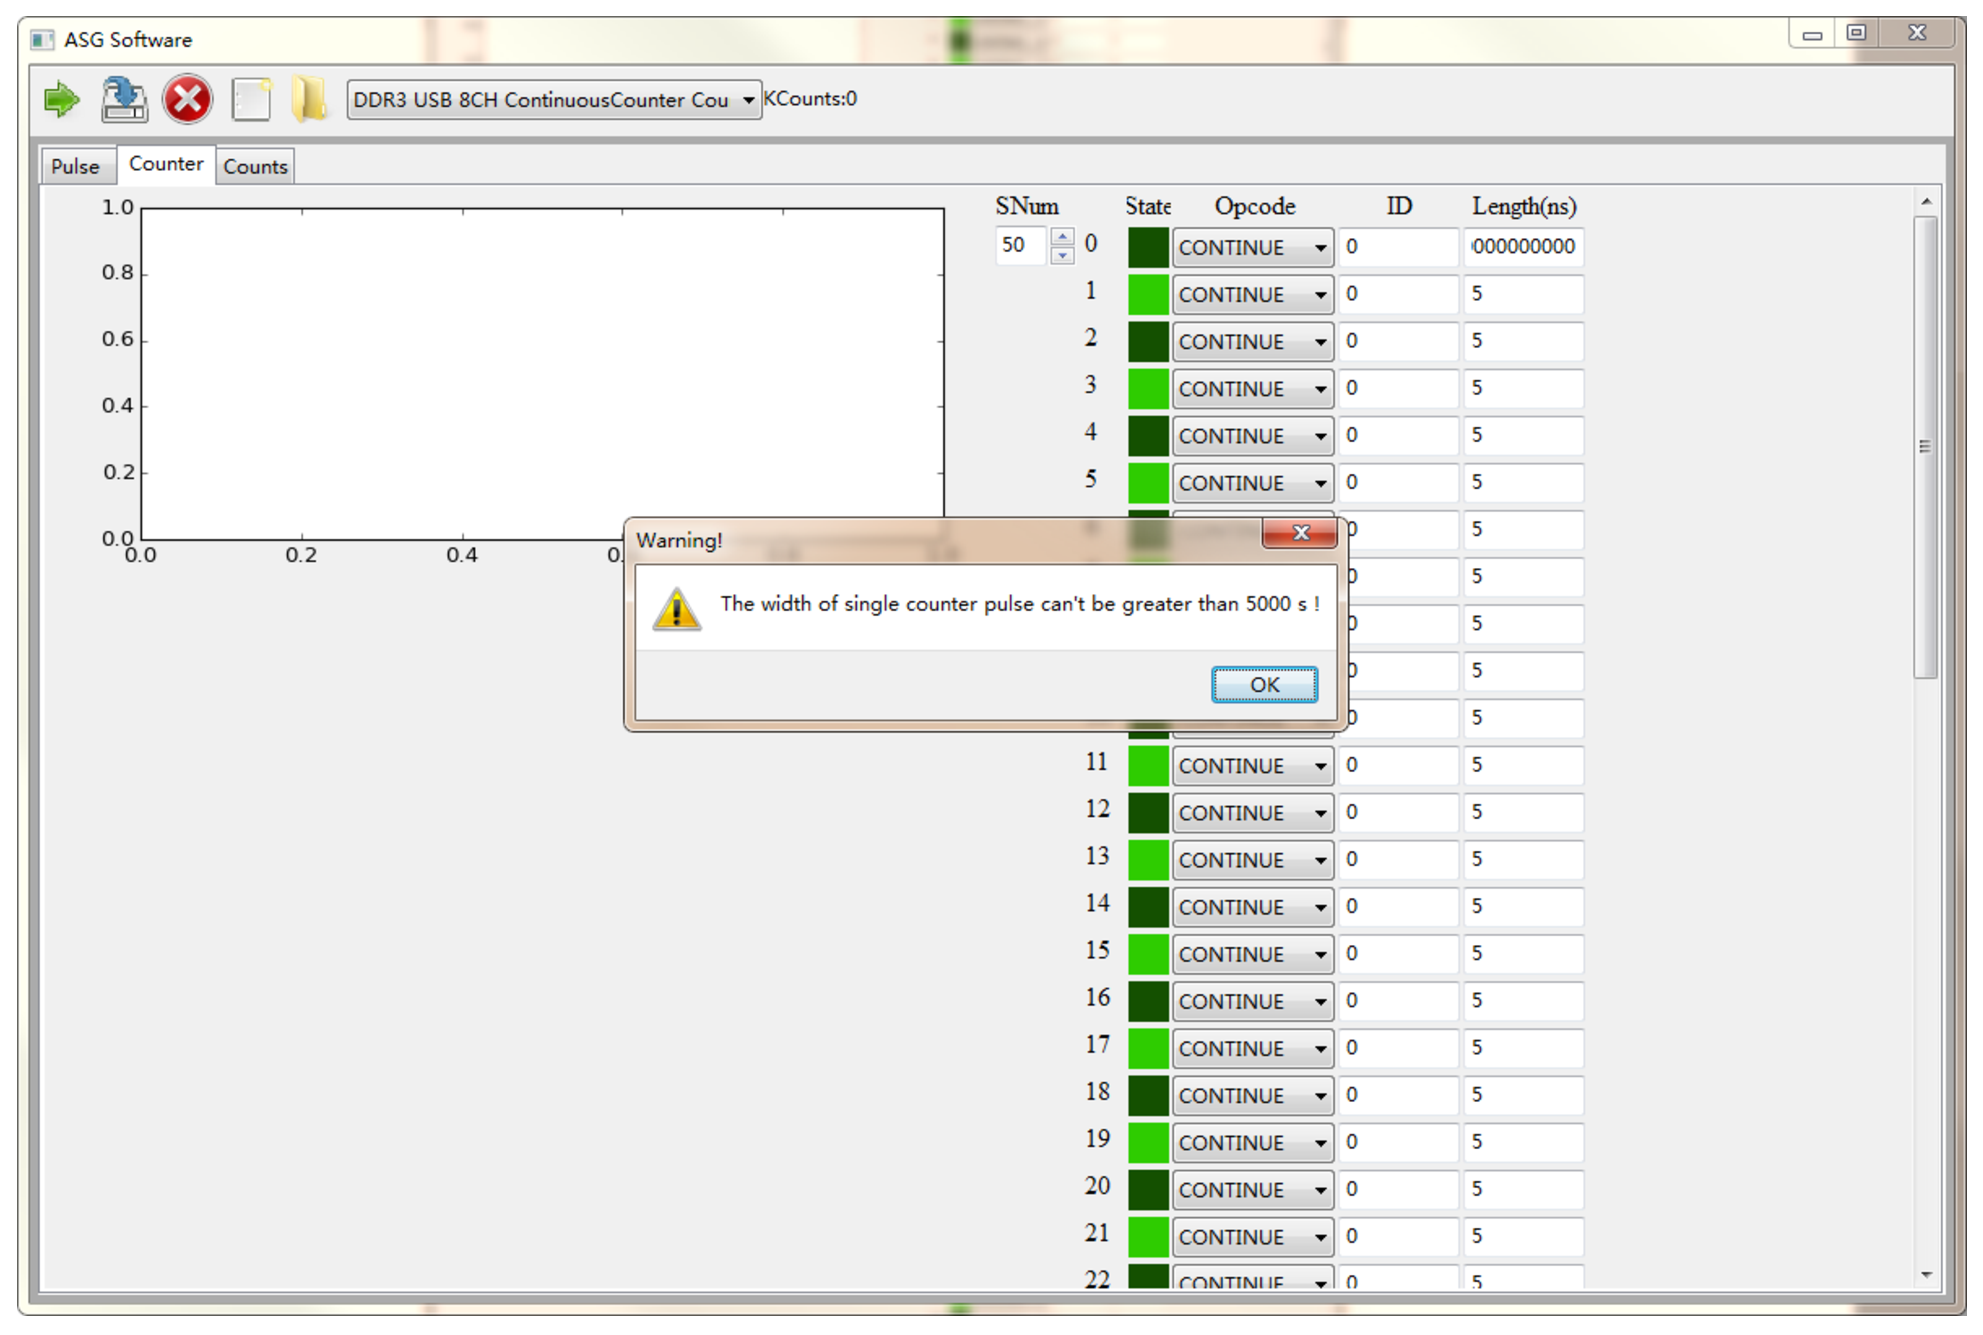
\includegraphics[height=8cm]{fig4_8}
\caption{宽度大于5000 s的非法计数通道使能序列输入}
\end{figure}

\noindent \textbf{(3)}.  用户定义的计数通道使能序列宽度必须是5 ns的整数倍,若存在非5 ns整数倍的情况,亦为非法输入,如图4.9。
\begin{figure}[ht]
\centering
%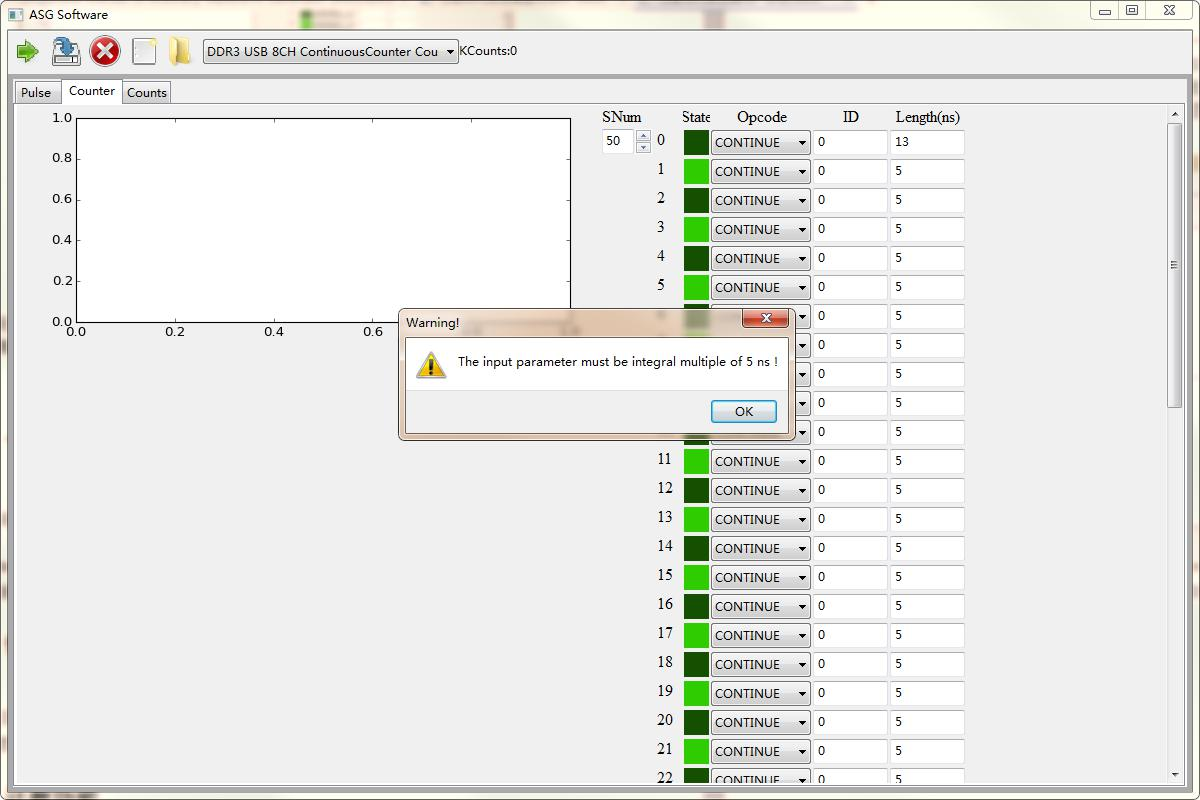
\includegraphics[width=10cm,height=7.5cm]{fig4_9}
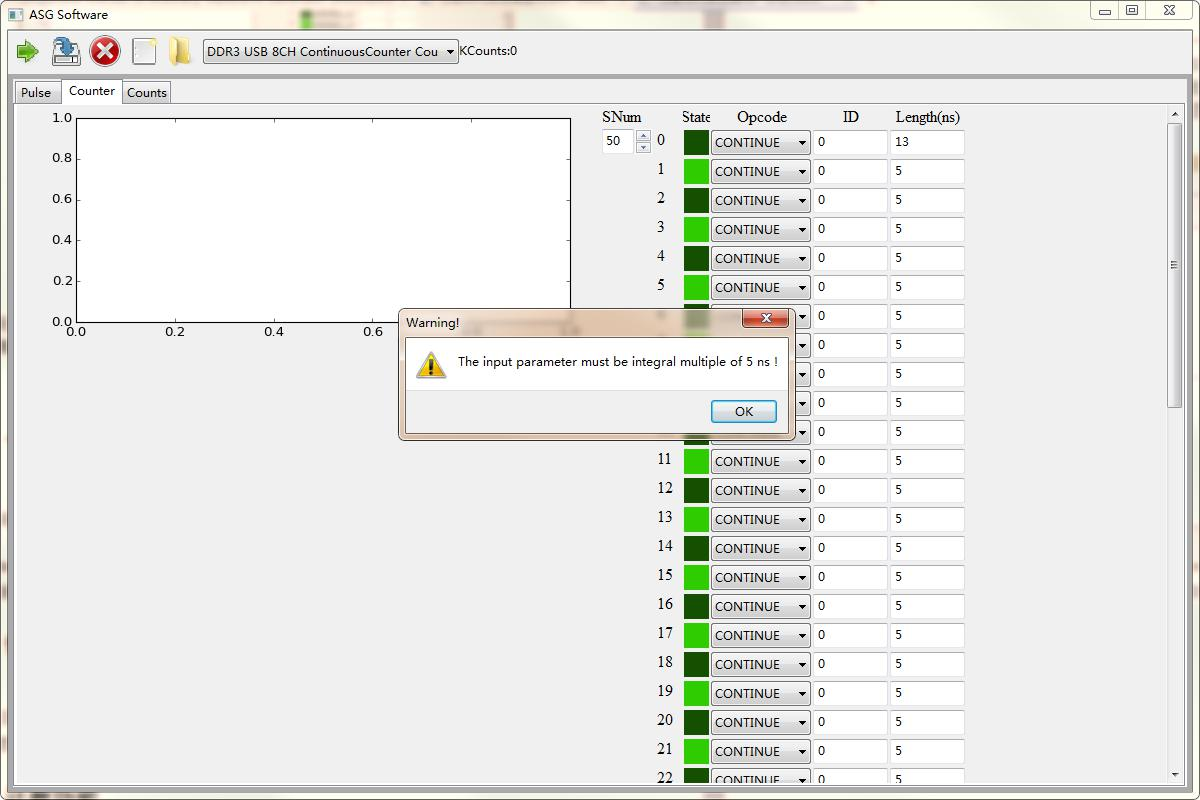
\includegraphics[height=8cm]{fig4_9}
\caption{宽度非5 ns整数倍的非法计数通道使能序列输入}
\end{figure}

\section{\heiti 开始计数与播放方波序列}
用户点击“Download”按钮

\includegraphics{download},可将自定义方波序列以及计数通道使能序列数据下载到硬件中。点击“Start”按钮

\includegraphics{start},可使仪器各输出通道开始同步播放自定义的方波序列并开始计数。将输出通道用同轴线接到示波器上可以看到输出的方波序列。

\section{\heiti 停止计数与播放方波序列}
当仪器正在计数并播放方波序列时,可以通过点击“Stop”按钮
\includegraphics{stop}使仪器停止计数并停止播放方波序列。

\section{\heiti 计数功能}
Counter的计数功能是指用户可以自定义计数通道使能序列,然后得到在计数通道使能序列高电平时间内输入信号的计数结果。当有外部信号输入计数通道时,用户可以在软件的Counter界面看到计数结果。计数结果显示在界面左侧的坐标图中。

\section{\heiti 周期计数功能}
周期计数功能是指用户可以利用软件连续获得一个周期(用户自定义)内的输入信号计数结果。周期计数功能主界面如图4.10所示。右侧文本输入框为用户自定义的周期计数时间(单位为秒),下方显示数字为输入计数通道内的信号频率(单位为kHz),左侧坐标图显示连续计数结果随时间的变化图。
\begin{figure}[ht]
\centering
%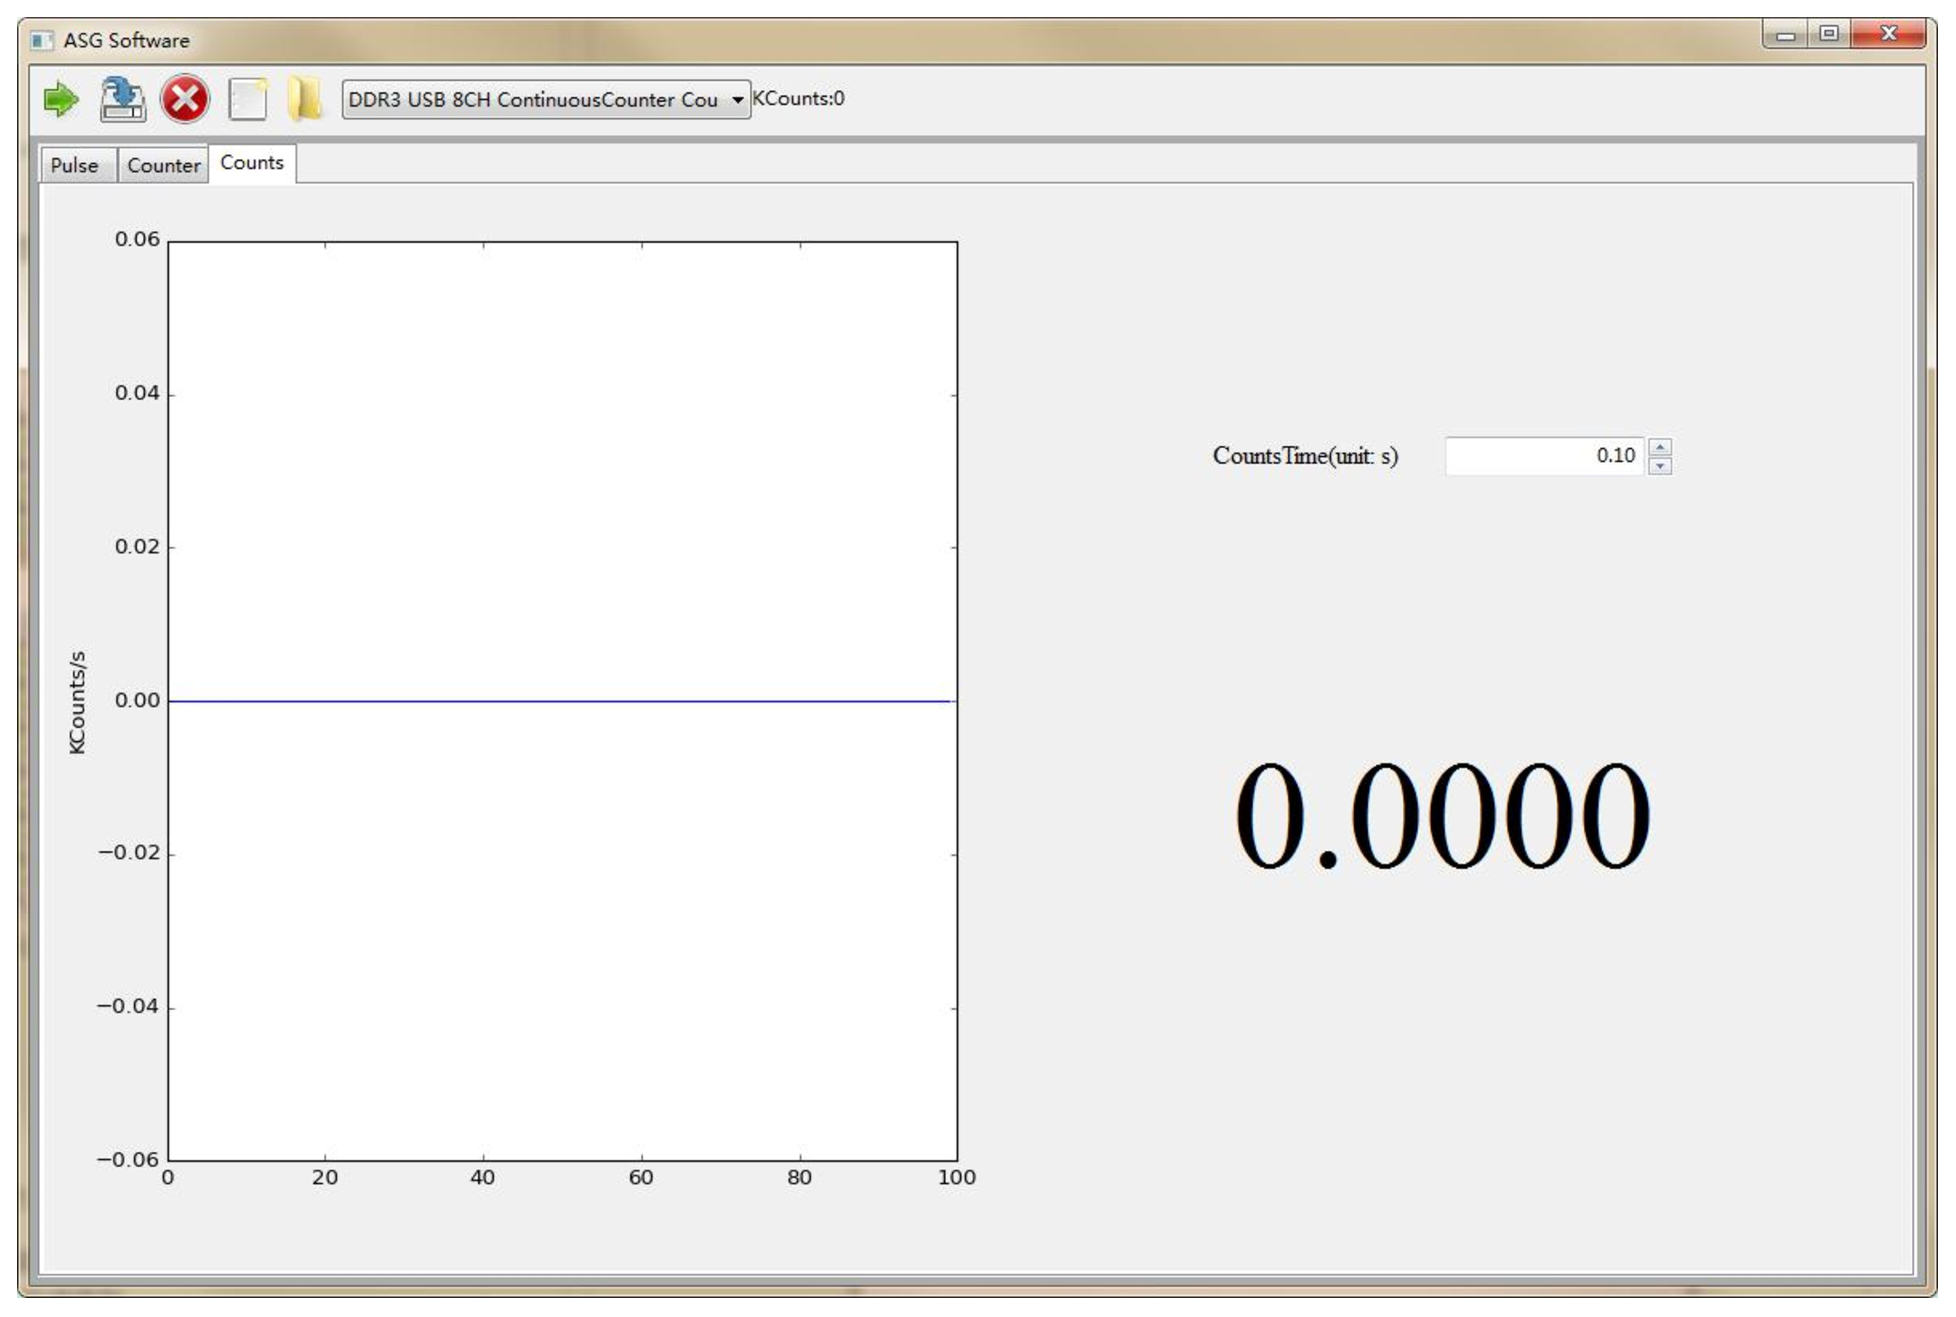
\includegraphics[width=10cm,height=7.5cm]{fig4_10}
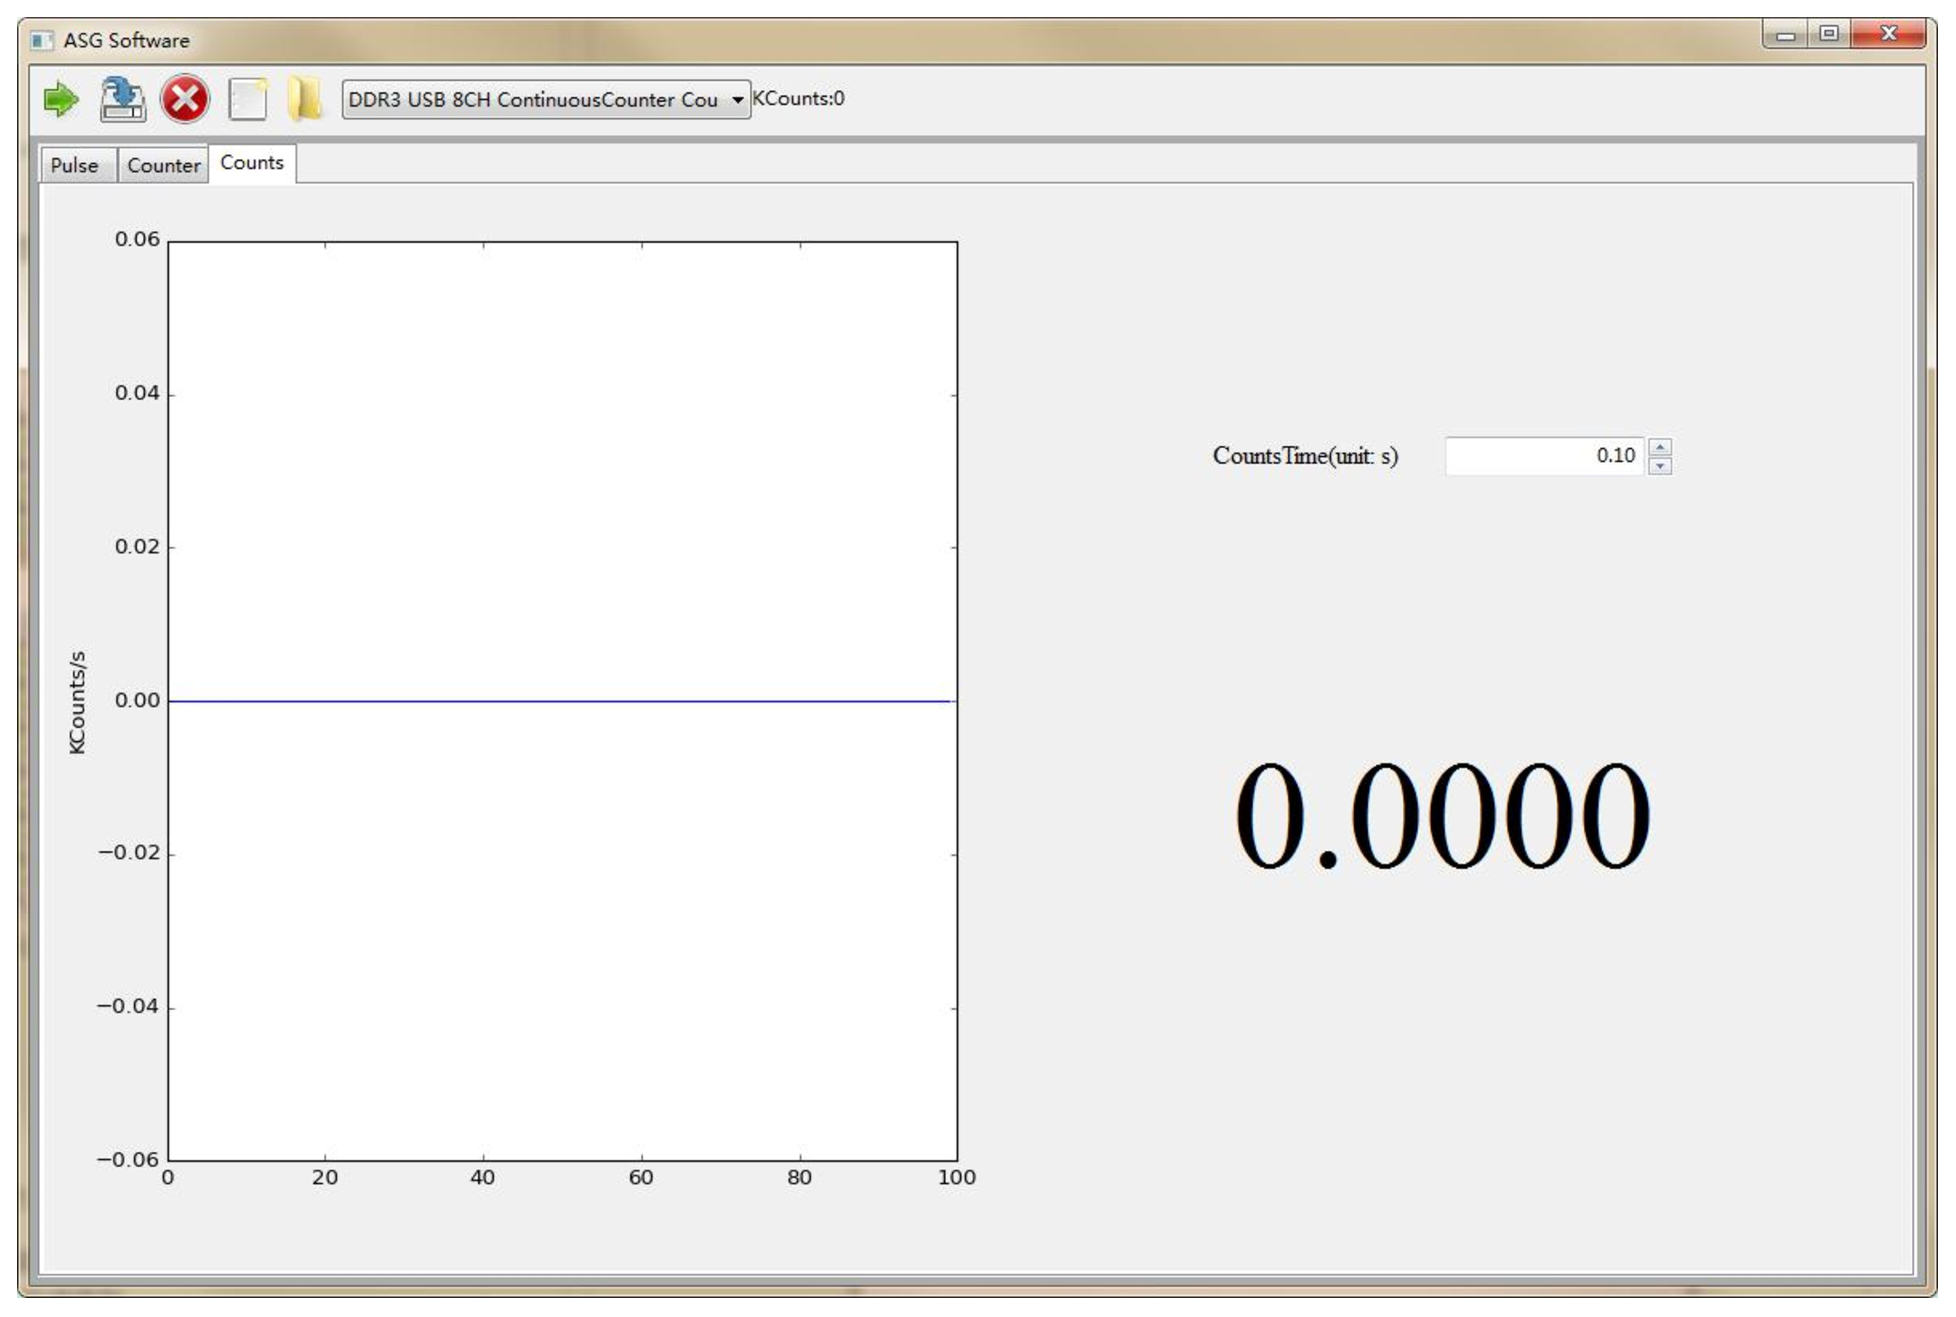
\includegraphics[height=9cm]{fig4_10}
\caption{周期计数主界面}
\end{figure}

